% !TEX root = ../XJ_thesis.tex
%
\chapter{Real-World Noisy Image Dataset: A New Benchmark}
\label{sec:dataset}

\section{Introduction}

During the past decades, the statistical property of realistic noise has been thoroughly studied for CCD and CMOS image sensors. As introduced previously in the INtroduction, the realistic noise related to the CCD or CMOS sensors could be divided into five major sources, including photon shot noise, fixed pattern noise, dark current, readout noise, and quantization noise, etc.

The shot noise is one inevitable source of noise and induced by the stochastic arrival process of photons to the sensor. This can be modeled by Possion process in which the number of photons arriving the sensor follows Possion distribution. This type of noise is proportional to the mean intensity of the specific pixel and is not stationary across the whole image. The fixed pattern noise include pixel response non-uniformity (PRNU) noise and dark current non-uniformity (DCNU) noise. PRNU means for a fixed light level, each pixel will have a slightly different output levels or responses. The major reason for the PRNU noise is the loss of light and color mixture in the neighboring pixels.

The dark current and fixed pattern noise are from the electronics within the sensor chip, while the readout noise and quantization noise are from discretization. The dark current is generated mainly  due to thermal agitation, even thouth there is no light reaching the camera sensor. The readout noise is mainly generated during the process of Charge-to-voltage conversion. The readout is inheretantly not accurate. This is also the reason for quantization noise, in which the readout value is quantizated to be an integer. The final pixel values are only discretization of the original raw pixel values. Other types of noise include CCD specific sources such as transfer efficiency and CMOS specific sources such as column noise.

As we have presented in the previous chapters, the image denoising task is very different in processing between realistic noise and the synthetic additive white Gaussian noise (AWGN). The realistic noise is signal dependent and will become much more complex when processed in the camera imaging pipeline, while the AWGN noise is independent of the signals. Hence, processing real noisy images is more challenging than the traditional AWGN noise.

Another issue about the realistic image denoising is how to evaluate the quality of the denoised images. The image quality assessment by subjective evaluation would be time-consuming since it needs enough subjectives to take part in the experiments. Short of subjectives would generate biased evaluation results. To alliviate this problem, an alternative way is to resort to the objective evaluation. However, the objective also has its own problems. Since the noisy images with realistic noise has no corresponding noise-free image, the objective evaluation on the quality of denoised images is very hard, not to say impossible. The missing of corresponding noise-free image to the realistic noisy image will be very problematic since we cannot perform objective measurements to evaluate the quality of the denoised image by the competing methods. And hence, we have no proper evaluation methods on the goodness of the proposed denoising methods.

In order to filling the gap of missing corresponding noise-free image to the captured realistic noisy image, we construct a large dataset including the realistic images with reasonably obtained corresponding noise-free images. The basic idea is to capture the same and unchanged scene for many (e.g., 500) times and compute their mean image, which can be roughly taken as the noise-free image for the realistic noisy images. The rational behind the activity is that for each pixel, the noise on it is generated randomly larger or smaller than the true pixel value, and taking the same pixel many times and compute the average value will approximate the truth pixel value and alleviate the randomness of the capturing process. This is inspired by the recent work of \cite{crosschannel2016}, in which a small dataset is constructed for analyzing the properties of realistic noise during the camera imaging pipeline. However, this dataset is limited in its contents. It contains only printed pictures on the package of several products, while has few real object of different kinds. Besides, the images in this dataset is not refined by suitable post-processing. Hence, the images and its corresponding noise-free images would exhibit spatial misalignment. Other problems may include that the intensity transform does not model heteroscedastic noise, and low-frequency bias is not removed, etc. Our experiments
indicate that ignoring these sources of error will significantly affects the realism of the dataset. Moreover, the images in the dataset \cite{crosschannel2016} are based on $8$-bit demosaiced images while we work with untainted linear raw intensities.

It is often useful to measure the noise characteristics of a sensor at a certain ISO level. \cite{} proposes to illuminate the sensor with approximately constant irradiation and subsequently aggregates intensity measurements spatially. This is repeated for different irradiation levels to capture the intensity dependence of the noise. \cite{} propose a less tedious capture protocol similar to ours, where multiple exposures of a static scene are used to aggregate the measurements at every pixel site temporally. In contrast, our Tobit regression allows to estimate the parameters of the noise process by having access to just two images.


\section{Existing Datasets}

Compared with the work dealing with the Gaussian noise, there are only several work focus on benchmarking the denoising methods on realistic noisy images \cite{RENOIR2014,crosschannel2016,dnd2017}. The first effort on constructing a dataset on real noisy images is the RENOIR dataset \cite{RENOIR2014}. It relies on taking sets of images of a static scene with different ISO values. However, the post-processing is less refined. Image pairs appear to exhibit spatial misalignment, the intensity transform does not model heteroscedastic noise, and low-frequency bias is not removed. In \cite{RENOIR2014}, experiments have been evaluated to validate that ignoring these sources of error significantly
affects the realism of the dataset. It is often useful to measure the noise characteristics of a sensor at a certain ISO level. \cite{RENOIR2014} proposes to illuminate the sensor with approximately constant irradiation and subsequently aggregates intensity measurements spatially. This is repeated for different irradiation levels to capture the intensity dependence of the noise. \cite{RENOIR2014} propose a less tedious capture protocol similar to ours, where multiple exposures of a static scene are used to aggregate the measurements at every pixel site temporally.

The second work in this direction is proposed in the \cite{crosschannel2016}, in which 11 static scenes are collected as a dataset including realistic noisy images. For each scene, 500 JPEG images are captured and the mean image of each scene is computed to generate the ground truth noise-free image. Using the mean of temporal images as noise-free image has also been employed in \cite{Liu2008,liupractical}. In this dataset, the images are with resolution $7630\times4912$ captured by Nikon D800 (ISO=1600, 3200, 6400), Nikon D600 (ISO=3200), and Canon 5D Mark III (ISO=3200). The major problems of this dataset is that the captured images are almost printed scenes, which share similar nosie statistical property. 

The third work in this direction is recently proposed in the \cite{dnd2017}. In contrast, \cite{dnd2017} employs the Tobit regression which allows to estimate the parameters of the noise process by having access to just two images. The proposed DND benchmark for denoising algorithms consists of 50 scenes selected from their captured images. In order to obviate the unrealistic setting by developing a methodology for benchmarking denoising techniques on real photographs. The authors in \cite{dnd2017} capture pairs of images with different ISO values and appropriately adjusted exposure times, where the nearly noise-free low-ISO image serves as reference. To derive the ground truth, careful post-processing is needed. They correct spatial misalignment, cope with inaccuracies in the exposure parameters through a linear intensity transform based on a novel heteroscedastic Tobit regression model, and remove residual low-frequency bias that stems, e.g., from minor illumination changes. They then capture a novel benchmark dataset, the Darmstadt Noise Dataset (DND) \cite{dnd2017}, with consumer cameras of differing sensor sizes. One interesting finding is that various recent techniques that perform well on synthetic noise are clearly outperformed by BM3D \cite{bm3d} on realistic photographs. This benchmark delineates realistic evaluation scenarios that deviate strongly from those commonly used in the scientific literature.


\section{The Proposed Dataset}

\subsection{Motivation}

In order to take more comprehensive comparison on the existing denoising methods, we propose to construct a new dataset which eliminates the problem mentioned above. The camera we use are the Canon 5D, Nikon D800, Olympus, and Sony A7II. The brands are more versatile than the above mentioned three datasets. In addition, we use the raw data of mobile phone. 

There are several problems hindering us from touching the raw data of mobile phone. The first one is that most mobile phones do not support the raw data output. Even the raw data of  iPhone is processed before being output, not the original one. Here, we use the raw data of the iPhone and process it for the final RGB images. The second problem is that it is hard to capture the static image with hundreds of repetition with mobile phone. The solution is that we can use apple watch to remote control the iPhone for image capturing. 

The format of our captured images are raw data and JPEG images with uncompressed process. For each scene, we capture it for 500 times, just as \cite{crosschannel2016} did. The focus is set by firstly automatic and then mannually when capturing the images. We capture the images indoor with normal lighting condition, dark lighting condition, and the outdoor normal lighting condition. The scenes we capture are also versaltile. The objects in our scene are objects like books, pens, bottles, and boxes, joys, etc. The places include the corner of building s, classrooms, the caffe rooms, and the outdoor places.

The camera settings are very important when we capture the realistic noisy images. In general, the smaller shutter, the darker the captured images, when we fix the other conditions, and vice versa. Similarly, the smaller ISO, the darker the captured images, when we fix the other conditions, and vice versa. In order to speed up the capturing process (shorten the capturing duration), the shutter should be set sa smaller as possible. In this case, the captured images would also be in least influenced by the environment. The shutter of the Sony A7II camera is between 1/80000 second to 30 seconds. Given suitable aperture and ISO, it is possible to capture images with normal illuminations when we set the shutter between 1/100 second and 1 second. The aperture could be set as any value only if it is in the reasonable region . The aperture of the Sony camera is between F3.5 and F22. Setting the aperture between F3.5 and F15 can help obtain the images with normal illumination under the fixed and suitable shutter and ISO. In our capturing process, we fixed the shutter and aperture to be in suitable and reasonable region, and tune the ISO values according to the reasonable region of the camera. In general, the noise level would be higher when the ISO is higher. It is helpful to the quantization and quantitation analysis if we set the ISO values from a low value to a high value with fixed gap.

To analysis how ISO, shutter, and aperture influence the content and illumination of the captured images, we perform some initial experiments. In Figure \ref{fig6-1}, we show some images captured with different camera settings. When comparing the Figures \ref{fig6-1}(a) and \ref{fig6-1}(b) (or \ref{fig6-1}(g) and \ref{fig6-1}(i)), we find that higher aperture indicate darker illumination. When comparing the Figures \ref{fig6-1}(b) and \ref{fig6-1}(c) (or \ref{fig6-1}(g) and \ref{fig6-1}(h)), we find that longer shutter indicate brighter illumination. When comparing the Figrues \ref{fig6-1}(b), \ref{fig6-1}(d), \ref{fig6-1}(e), \ref{fig6-1}(f), and \ref{fig6-1}(g), we find that the illumination would be brighter when the ISO is higher. Besides, given fixed aperture and shutter, the images captured by the camera can avoid the overexposure or underexposure when the ISO is set between 400 and 3200.  When ISO=200, the captured images would have the problem of underexposure, while when ISO=6400, the captured images would have the problem of overexposure. However, this can be alliviated by changing the aperture and shutter and finally we can obatian the images with normal illuminations.

Given fixed amount of exposure and aperture, enhancing the camera sensitivity will generate higher noise levels than lowering the shutter speed. When we build up the dataset, we only change the ISO values while fixing shutter and aperture with suitable values. The images will not suffer overexposure or underexposure with suitable ISO values. It is commonly accepted that the noise in images will become larger when the scene is under darker light source under the fixed camera setting.


\begin{figure}
    \centering
    \begin{subfigure}[t]{0.32\textwidth}
        \centering
        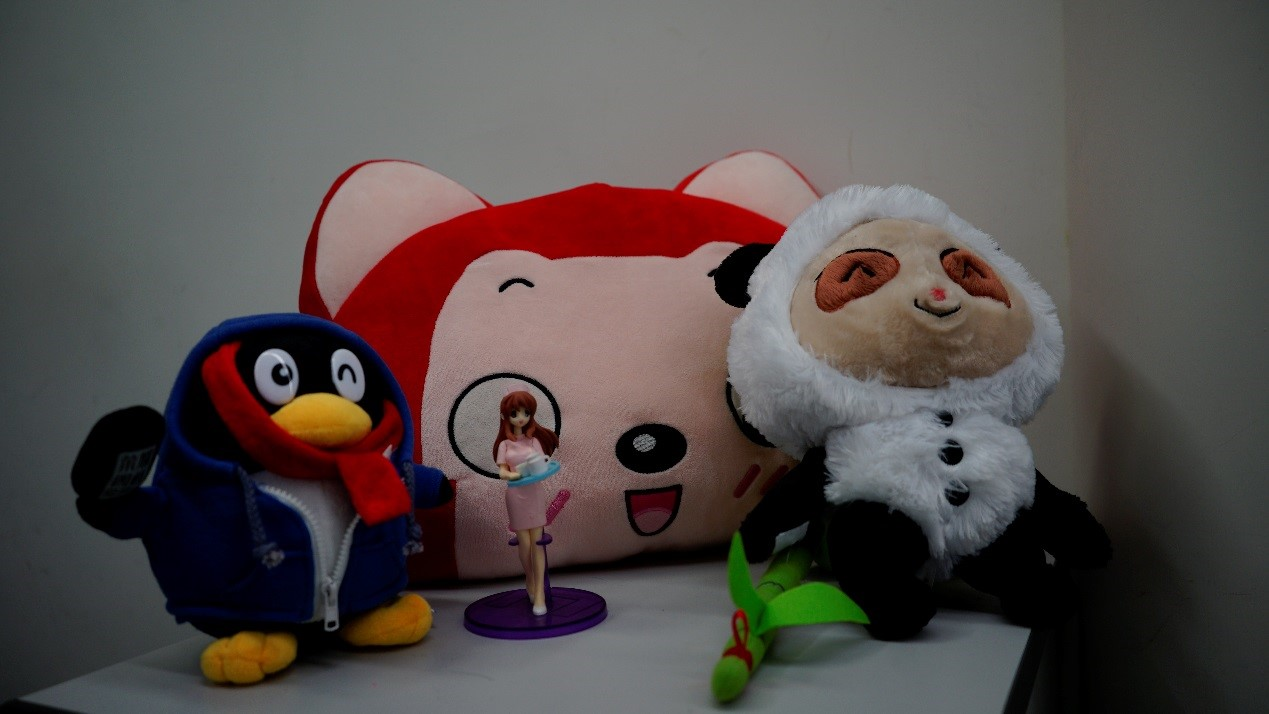
\includegraphics[width=1\textwidth]{images/dataset/200_3-5_1-60.jpg}
	   \caption{200,3.5,1/60}
    \end{subfigure}
    \hfill
    \begin{subfigure}[t]{0.32\textwidth}
        \centering
        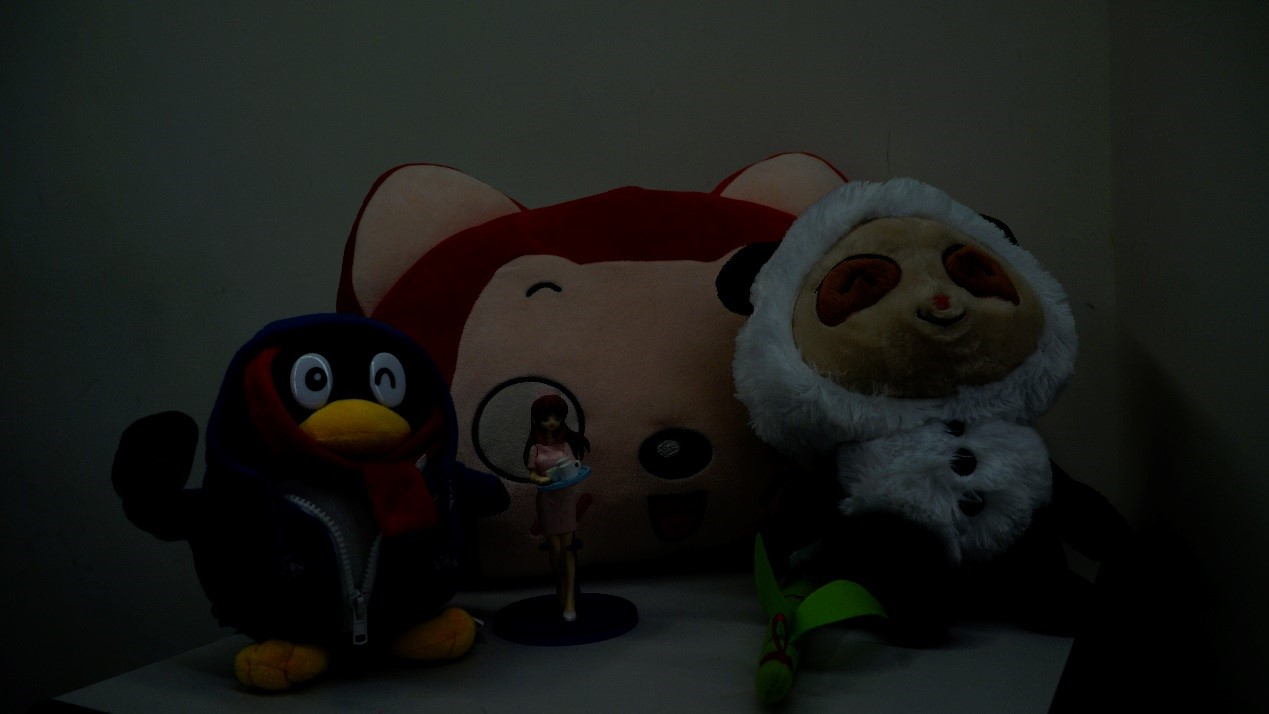
\includegraphics[width=1\textwidth]{images/dataset/200_6-7_1-60.jpg}
		\caption{200,6.7,1/60}
    \end{subfigure}
    \hfill
    \begin{subfigure}[t]{0.32\textwidth}
        \centering
        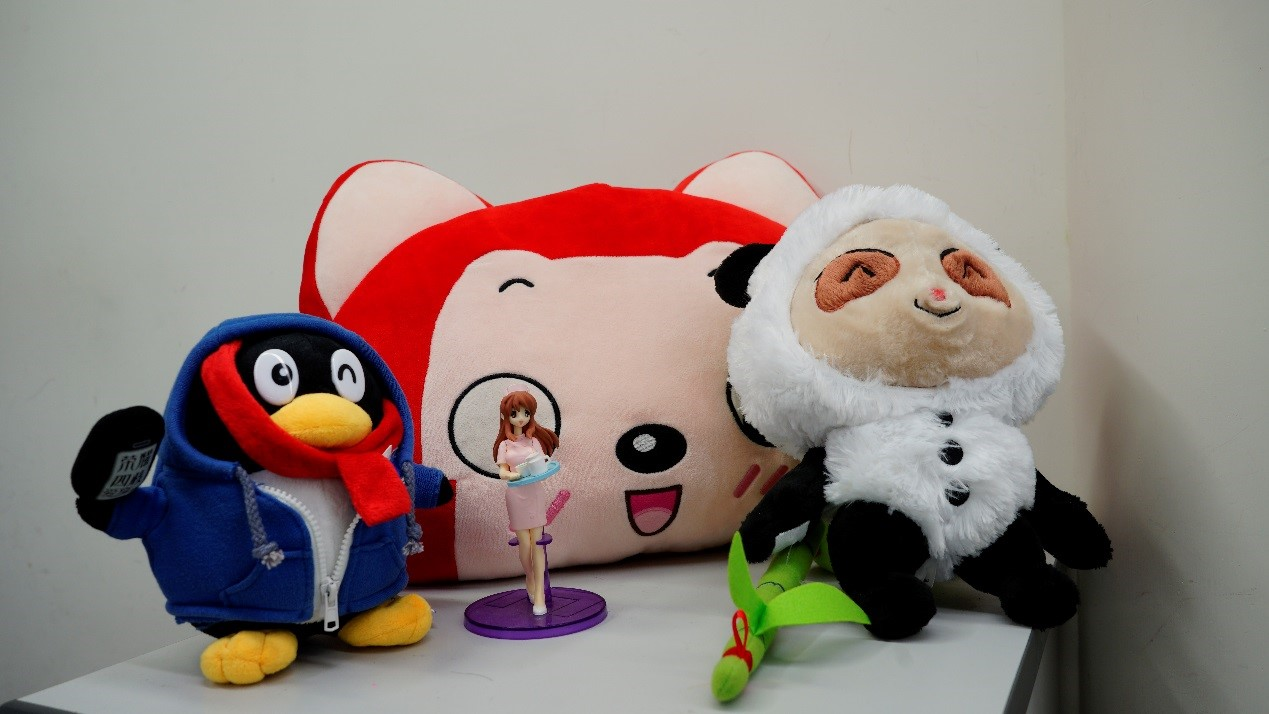
\includegraphics[width=1\textwidth]{images/dataset/200_6-7_1-8.jpg}
		\caption{200,6.7,1/8}
    \end{subfigure}
    \hfill
    \begin{subfigure}[t]{0.32\textwidth}
        \centering
        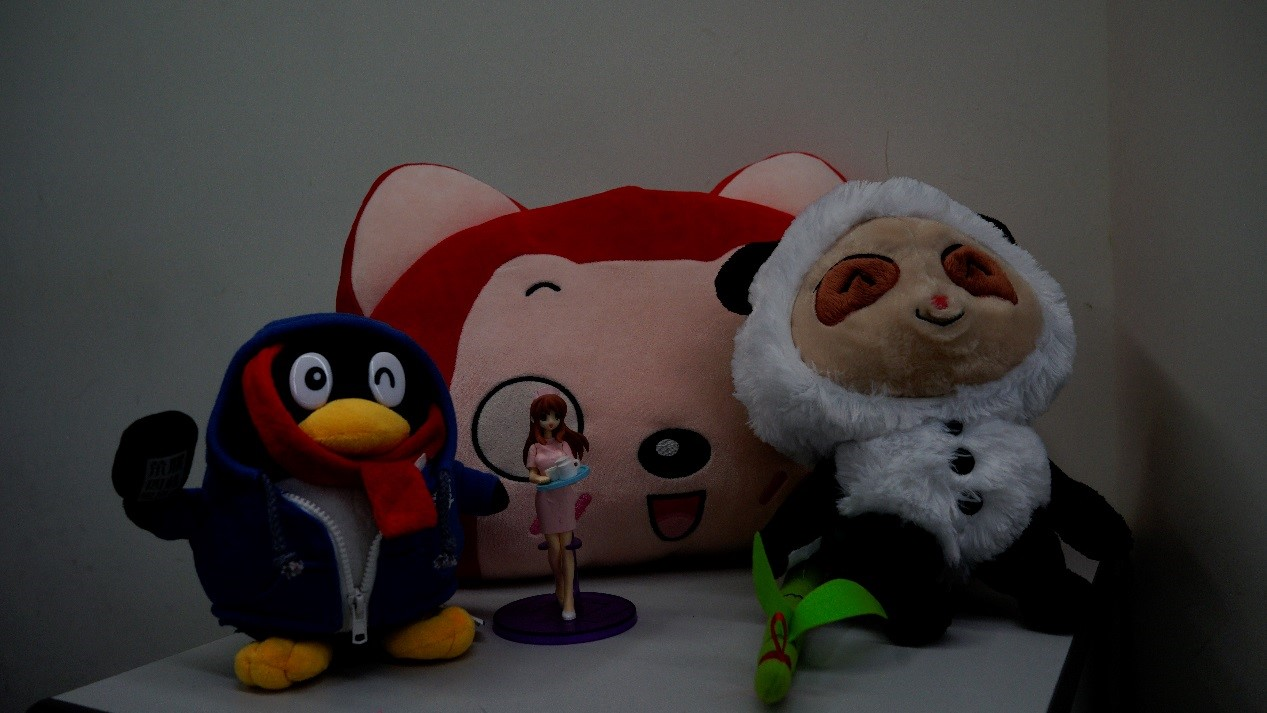
\includegraphics[width=1\textwidth]{images/dataset/400_6-7_1-60.jpg}
		\caption{400,6.7,1/60}
    \end{subfigure}
    \hfill
    \begin{subfigure}[t]{0.32\textwidth}
        \centering
        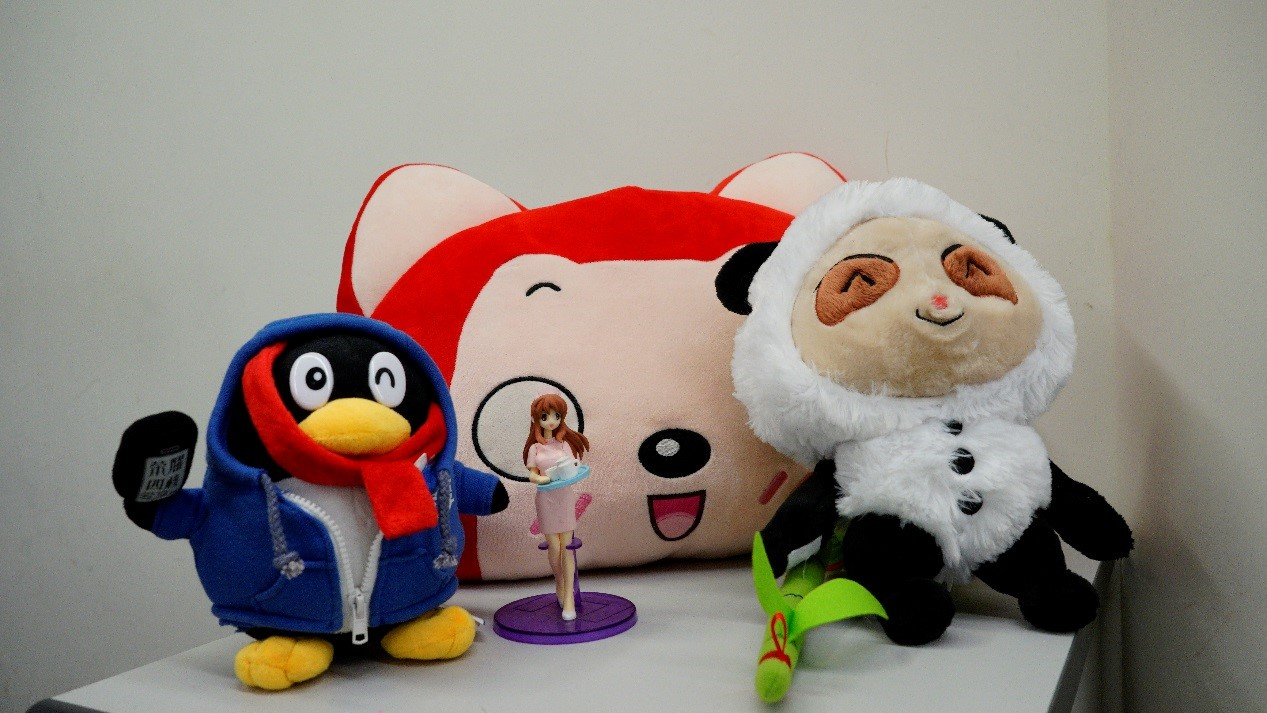
\includegraphics[width=1\textwidth]{images/dataset/1600_6-7_1-60.jpg}
		\caption{1600,6.7,1/60}
    \end{subfigure}
    \hfill
    \begin{subfigure}[t]{0.32\textwidth}
        \centering
        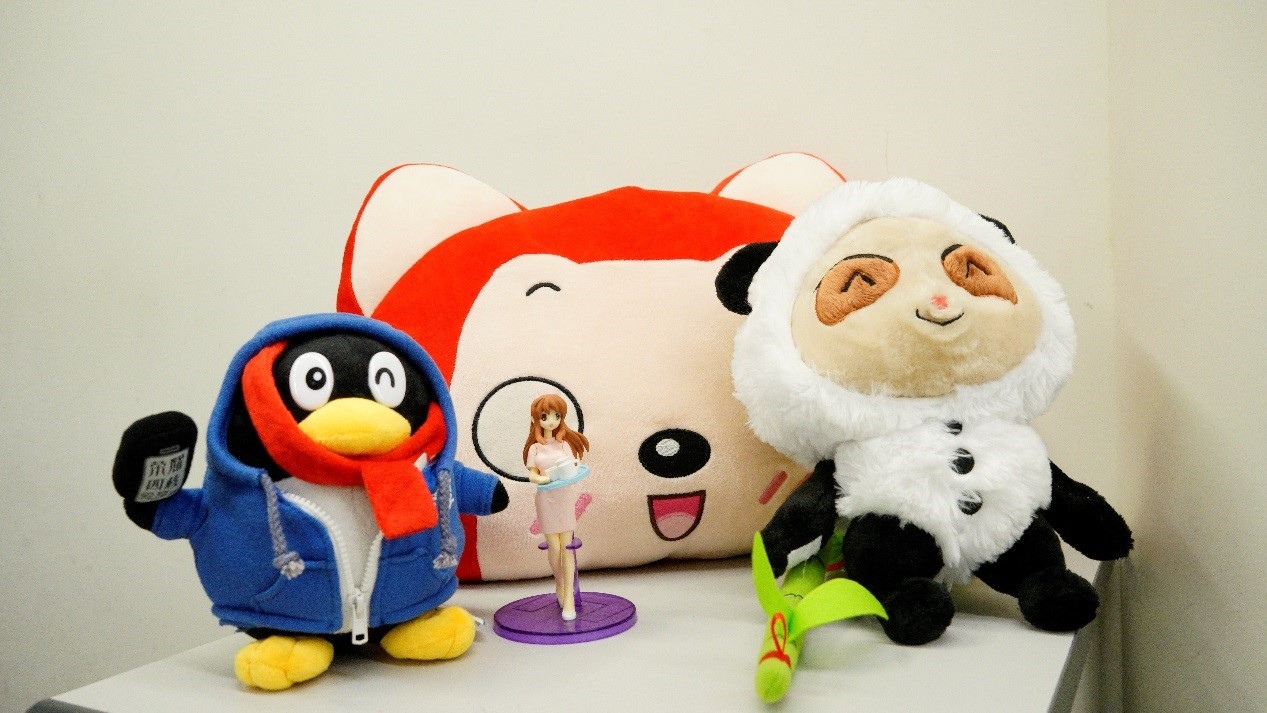
\includegraphics[width=1\textwidth]{images/dataset/3200_6-7_1-60.jpg}
		\caption{3200,6.7,1/60}
    \end{subfigure}
    \hfill
    \begin{subfigure}[t]{0.32\textwidth}
        \centering
        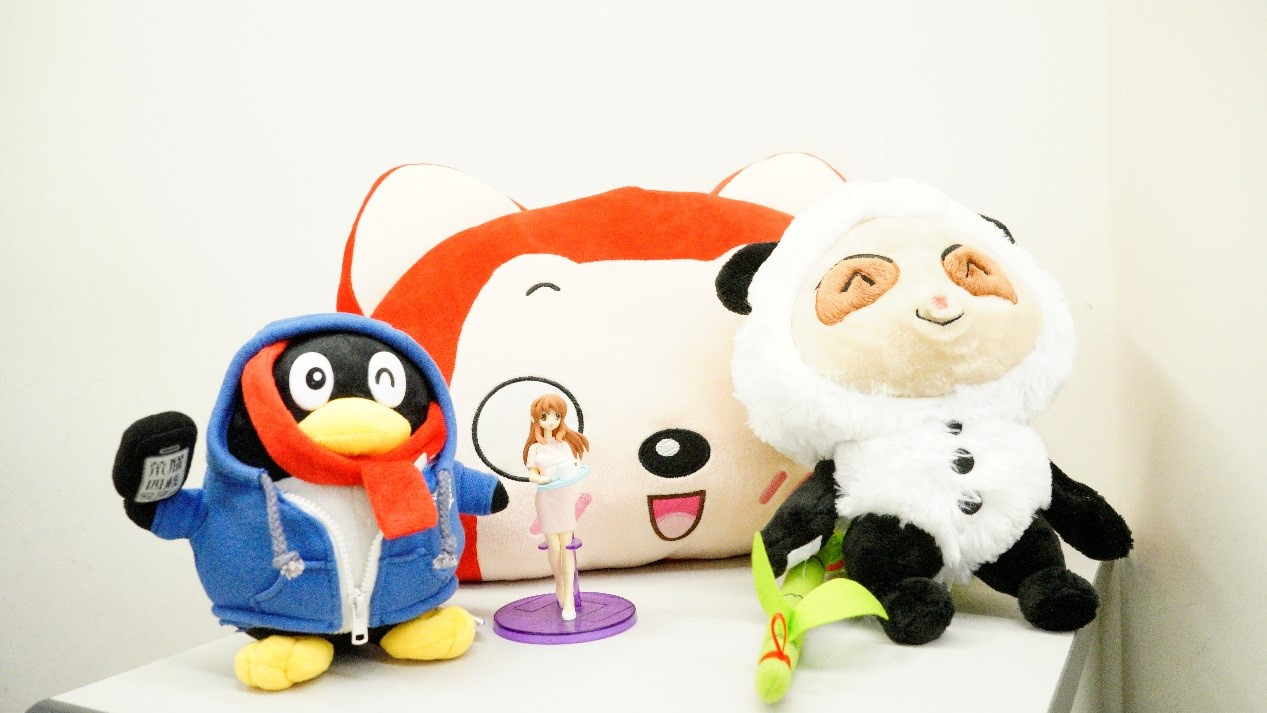
\includegraphics[width=1\textwidth]{images/dataset/6400_6-7_1-60.jpg}
		\caption{6400,6.7,1/60}
    \end{subfigure}
    \hfill
    \begin{subfigure}[t]{0.32\textwidth}
        \centering
        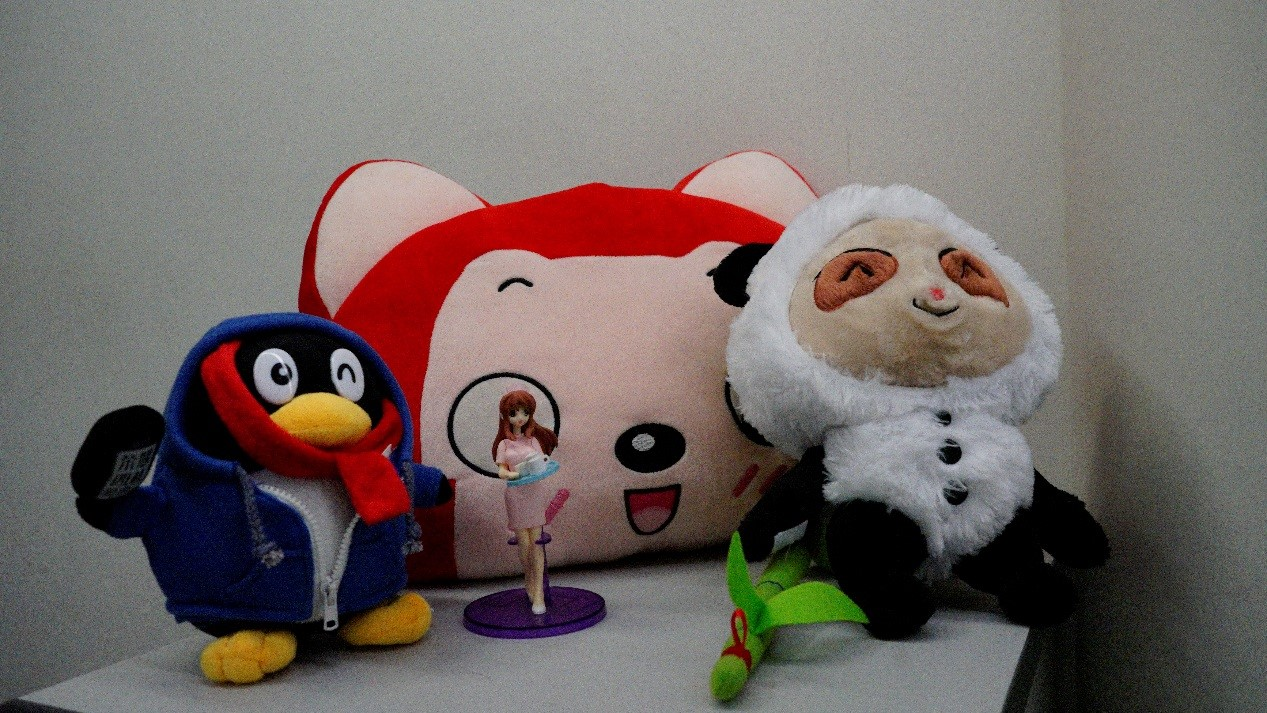
\includegraphics[width=1\textwidth]{images/dataset/6400_6-7_1-350.jpg}
		\caption{6400,6.7,1/350}
    \end{subfigure}
    \hfill
    \begin{subfigure}[t]{0.32\textwidth}
        \centering
        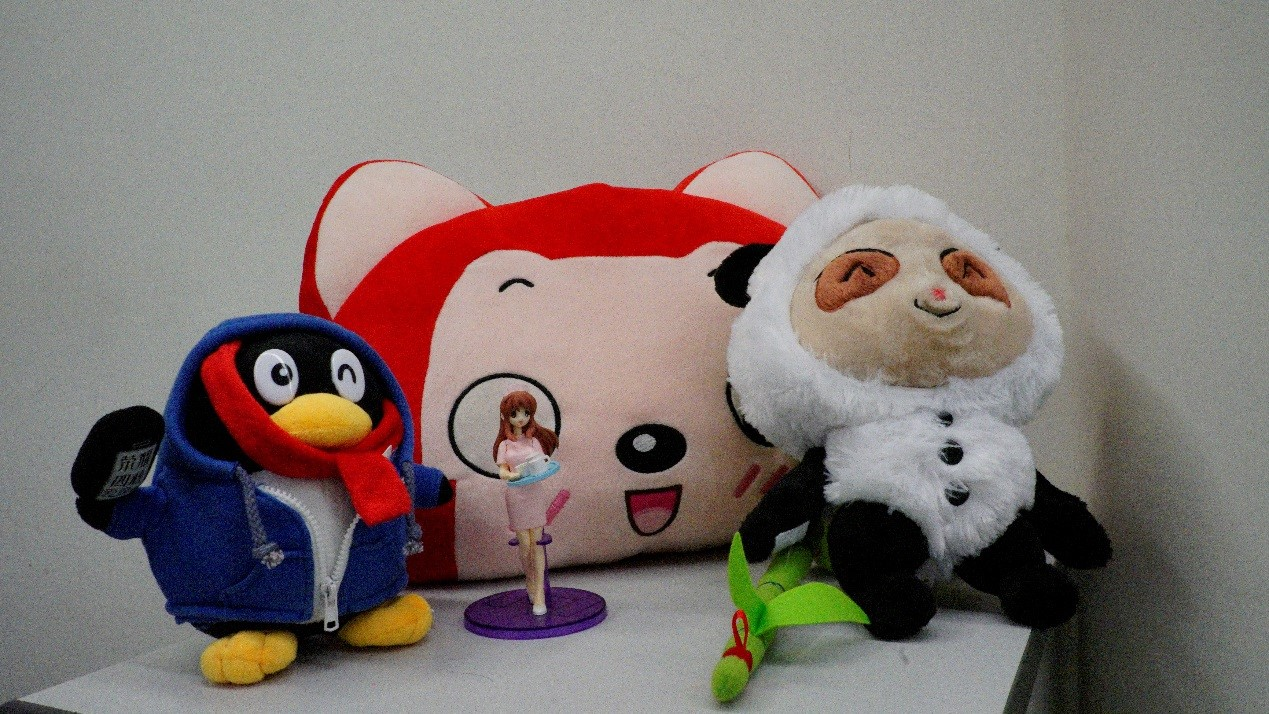
\includegraphics[width=1\textwidth]{images/dataset/6400_16_1-60.jpg}
		\caption{6400,16,1/60}
    \end{subfigure}
    \caption{Captured Images with the Sony A7 II camera under different (ISO, Shutter, Aperture) settings.}
    \label{fig6-1}
\end{figure}


\subsection{The Construction Process}

To alleviate the limitations of the previous dataset, we propose to further construct a new dataset which are: 1) contains more camera brands with more realistic noise sources;  2) capture the images with more camera settings; 3) capture more realistic scenes with real objects; 4) capture both the raw data and sRGB data for comparison analysis on the noise. In the following we will discuss each advantages in detail.

\textbf{More Camera Brands}: The RENOIR dataset \cite{RENOIR2014} contains only the Canon camera (T3i and S90) and the mobile brand Xiaomi Mi3 for image collection. This dataset only contains one camera brand and one mobile brand. The dataset in \cite{crosschannel2016} contains two camera brands including Canon (5D) and Nikon (D600 and D800). The DND dataset \cite{dnd2017} employs cameras of Sony (A7R and RX100 IV),  Olympus (E-M10), and Huawei (Nexus 6P).

In our dataset, we choose three most commonly used camera brands, including Canon (5D), Nikon (D800), and Sony (A7II), to capture our realistic noisy images. According to a recent survey \cite{commoncamera}, the three camera brands occupy 48 of 50 most commonly used camera-lens combinations. The other two positions are from the camera brands of Fujifilm and Olympus. Hence, we believe that our dataset is more representive than the previous datasets.

\textbf{More Camera Settings}: In the RENOIR dataset \cite{RENOIR2014}, the reference images are all captured when the ISO=100. The ISO in noisy images are set as follows:  for Xiaomi Mi3, the ISO is set as 1600 or 3200; for Canon S90, the ISO is set as 640 or 1000; for Canon T3i, the ISO is set as 3200 or 6400. For all the cases except for the reference image of Canon S90, the exposure time are set as automatic. For Canon S90, the exposure time is set as 3.2 seconds. In the dataset \cite{crosschannel2016}, three different ISOs (e.g., 1600, 3200, and 6400) are employed when capturing images with Nikon D800, while ISO=3200 is utilized for Canon 5D and Nikon D600. The DND dataset \cite{dnd2017} contains ISOs of large range. The ranges of ISO are $100\sim25600$ for Sony A7R, $200\sim25600$ for Olympus E-M10, $125-8000$ for Sony RX100 IV, and $100\sim6400$ for Huawei Nexus 6P, respectively. 

In our newly constructed dataset, we capture images with 5 different ISOs with each camera, e.g., 800, 1600, 3200, 6400, 12800, and 25600. Besides, we take deep analysis on the shutter speed and aperture, and finally choose the most suitable camera setting. With the increasing of the ISO, the noise levels will also increase at the same scene we capture. Hence, our dataset is more comprehensive at the noise levels the the previous datasets. To make the images captured with ISO=25600 more naturally, we set the shutter speed to 1/320 second and aperture to F10.0. 

\textbf{More Realistic Scenes}: The RENOIR dataset \cite{RENOIR2014} capture 40 scenes for each camera brand, and the overall 120 scenes are included in the dataset.  The dataset \cite{crosschannel2016} contains only 11 indoor scenes, in which the 11 scenes are overlapped on partial contents and objects. 

\textbf{Removing Outlier Images.} The outlier images are those images with misalignment with the base image (we usually choose the first image as the base image), and the images with different illuminance. In the dataset of \cite{crosschannel2016}, the authors did not consider to remove the images with misalignment and different illuminances. In the DND dataset \cite{dnd2017}, the authors considered to correct the misalignment of each image. However, the correction largely depends on the misalignment detection method and the correction also largely dependens on the other methods, which will make the corrected images not as naturally as the images naturally captured by the cameras. Besides, the DND dataset \cite{dnd2017} view the image captured with low ISO value as ``ground truth'', and linearly transfer the noisy image captured with high ISO value to the scale of the ``ground truth'' image. This step, in our opinion, is problematic since the image pixels are not strictly linear dependent to the ISO values. 
 
\textbf{Ground Truth Image Generation}: The ``Ground Truth'' images of the RENOIR dataset \cite{RENOIR2014} is generated when the camera is set with ISO=100 while the other settings are the same with the noisy images. The ``Ground Truth'' images of the dataset \cite{crosschannel2016} are generated by averaging the static images captured on the same scene under the same camera settings. The ``Ground Truth'' images of the DND dataset \cite{dnd2017} is also generated mainly by capturing the clean images with low ISO values (e.g., ISO=100), other post-processing steps include   linear intensity changes, spatial misalignment, and low-frequency residual correciton, etc. In our dataset, we employ the method of \cite{crosschannel2016} due to its simplisity. We just capture the same static scenes for many ($500\sim1000$) times and average the captured images to get the clean ``Ground Truth'' images.
 
\subsection{Summary of the Dataset}

We capture images with different camera settings. The cameras are set based on the following rules: the first rule is that the exposure time should be larger than the blink of the fluorescent lights, otherwise the flickering of the light will make the global illuminances of the captured images very different. The second rule is that we should set the shutter speed, the exposure time, and the ISO value accordingly so that the scenes are in a naturally lighting condition. Besides, since the DSLRs use mechanical shutter, the exposure time of each shot is irregular. This small error results in the different brightness of shots. However, we ignored this error in our dataset, so as the \cite{crosschannel2016}.

We first remove the images with unalignment with carefully subjective evaluation. The images with several pixels movement will be deleted. After this first filtering, we will then remove the images with inconsistant illuminance. The illuminance is generated by two reasons. One is that the captured scenes are influenced by the lighting conditions of the environment. The other is that the camera will automatically make up the illuminance when the scene are in a relatively low lighting condition. This is because we capture images for many times, and some of them may have different illumination, though captured under the same lighting condition. To remove the images with different illuminance, we first uniformly sample 10000 pixels ($100\times100$) in the image, and then compute their mean illuminances. Each of the captured images we captured will have one value representing its mean illuminances. We sort these values in a decreasing order. The images with the lowest or highest mean illuminances will be refered as outlier images. We will remove these images until the lowest and highest mean illuminances are close to the ``center'' of the mean illuminances. Here, ``center'' means the middle of the sorted mean values or mean illuminances. In this way, the images which are darker or brighter than the image with the mean illuminance will be removed and the remaining images are very close to each other. Then the remaining images will be averaged to obtain the mean image, which will be used as the ``ground truth'' image. We believe these two steps are very important for constructing a better realistic dataset.


\textbf{Dataset Collection Information:} 
%Some information of the proposed dataset are listed in Table \ref{tab6-1}. 

In summary, we capture totqally 40 different scenes by using 5 different cameras in several different camera settings, including 12 scenes by 5D Mark II, 5 scenes by Canon 80D, 3 scens by Canon 600D, 13 scenes by Nikon D800, 7 scens by Sony A7II. Since the images are of large size ($3000\times3000$), we crop some region from these images and finnaly obtain 100 images of size $512\times512$. The 100 cropped images are captured by different cameras with different camera settings. These differences include long range ISO values from 1600 to 12800. To compensate the illuminance, we also set suitable shetter speed and aperture accordingly. 

\textbf{Examples of The Proposed Dataset:} In Figure \ref{fig6-2}, we show some samples of the realistic noisy images we captured in our new dataset. From which we can see that the scenes we captured are much more complex and comprehensive than the previous datasets. For example, we captured the scenes from different types of classrooms, various types of indoor scenes, and versaitile objects under fixed lighting conditions, etc. These scenes are largely different from the scenes of previous datasets. We choose images those look typically for daily photograpy, or those including regions which we believe to be challenging for the image denoising methods. 

Since the images we captured are in very large size, we crop 100 smaller parts from the 40 scenes to evaluated the existing image denoising methods. Some examples of the cropped parts and their corresponding ``ground truth'' images are listed in Figure \ref{fig6-3}. One can see that the cropped parts can represente the captured images in the whole dataset. Besides, one can see ththe ``ground truth'' image parts are clearly demonstrate the noise is removed from the corresponding cropped image parts. Hence, it is reasonable to emply this newly constructed dataset for evaluating the image denoising methods.


\begin{figure}
    \centering
    \begin{subfigure}[t]{0.32\textwidth}
        \centering
        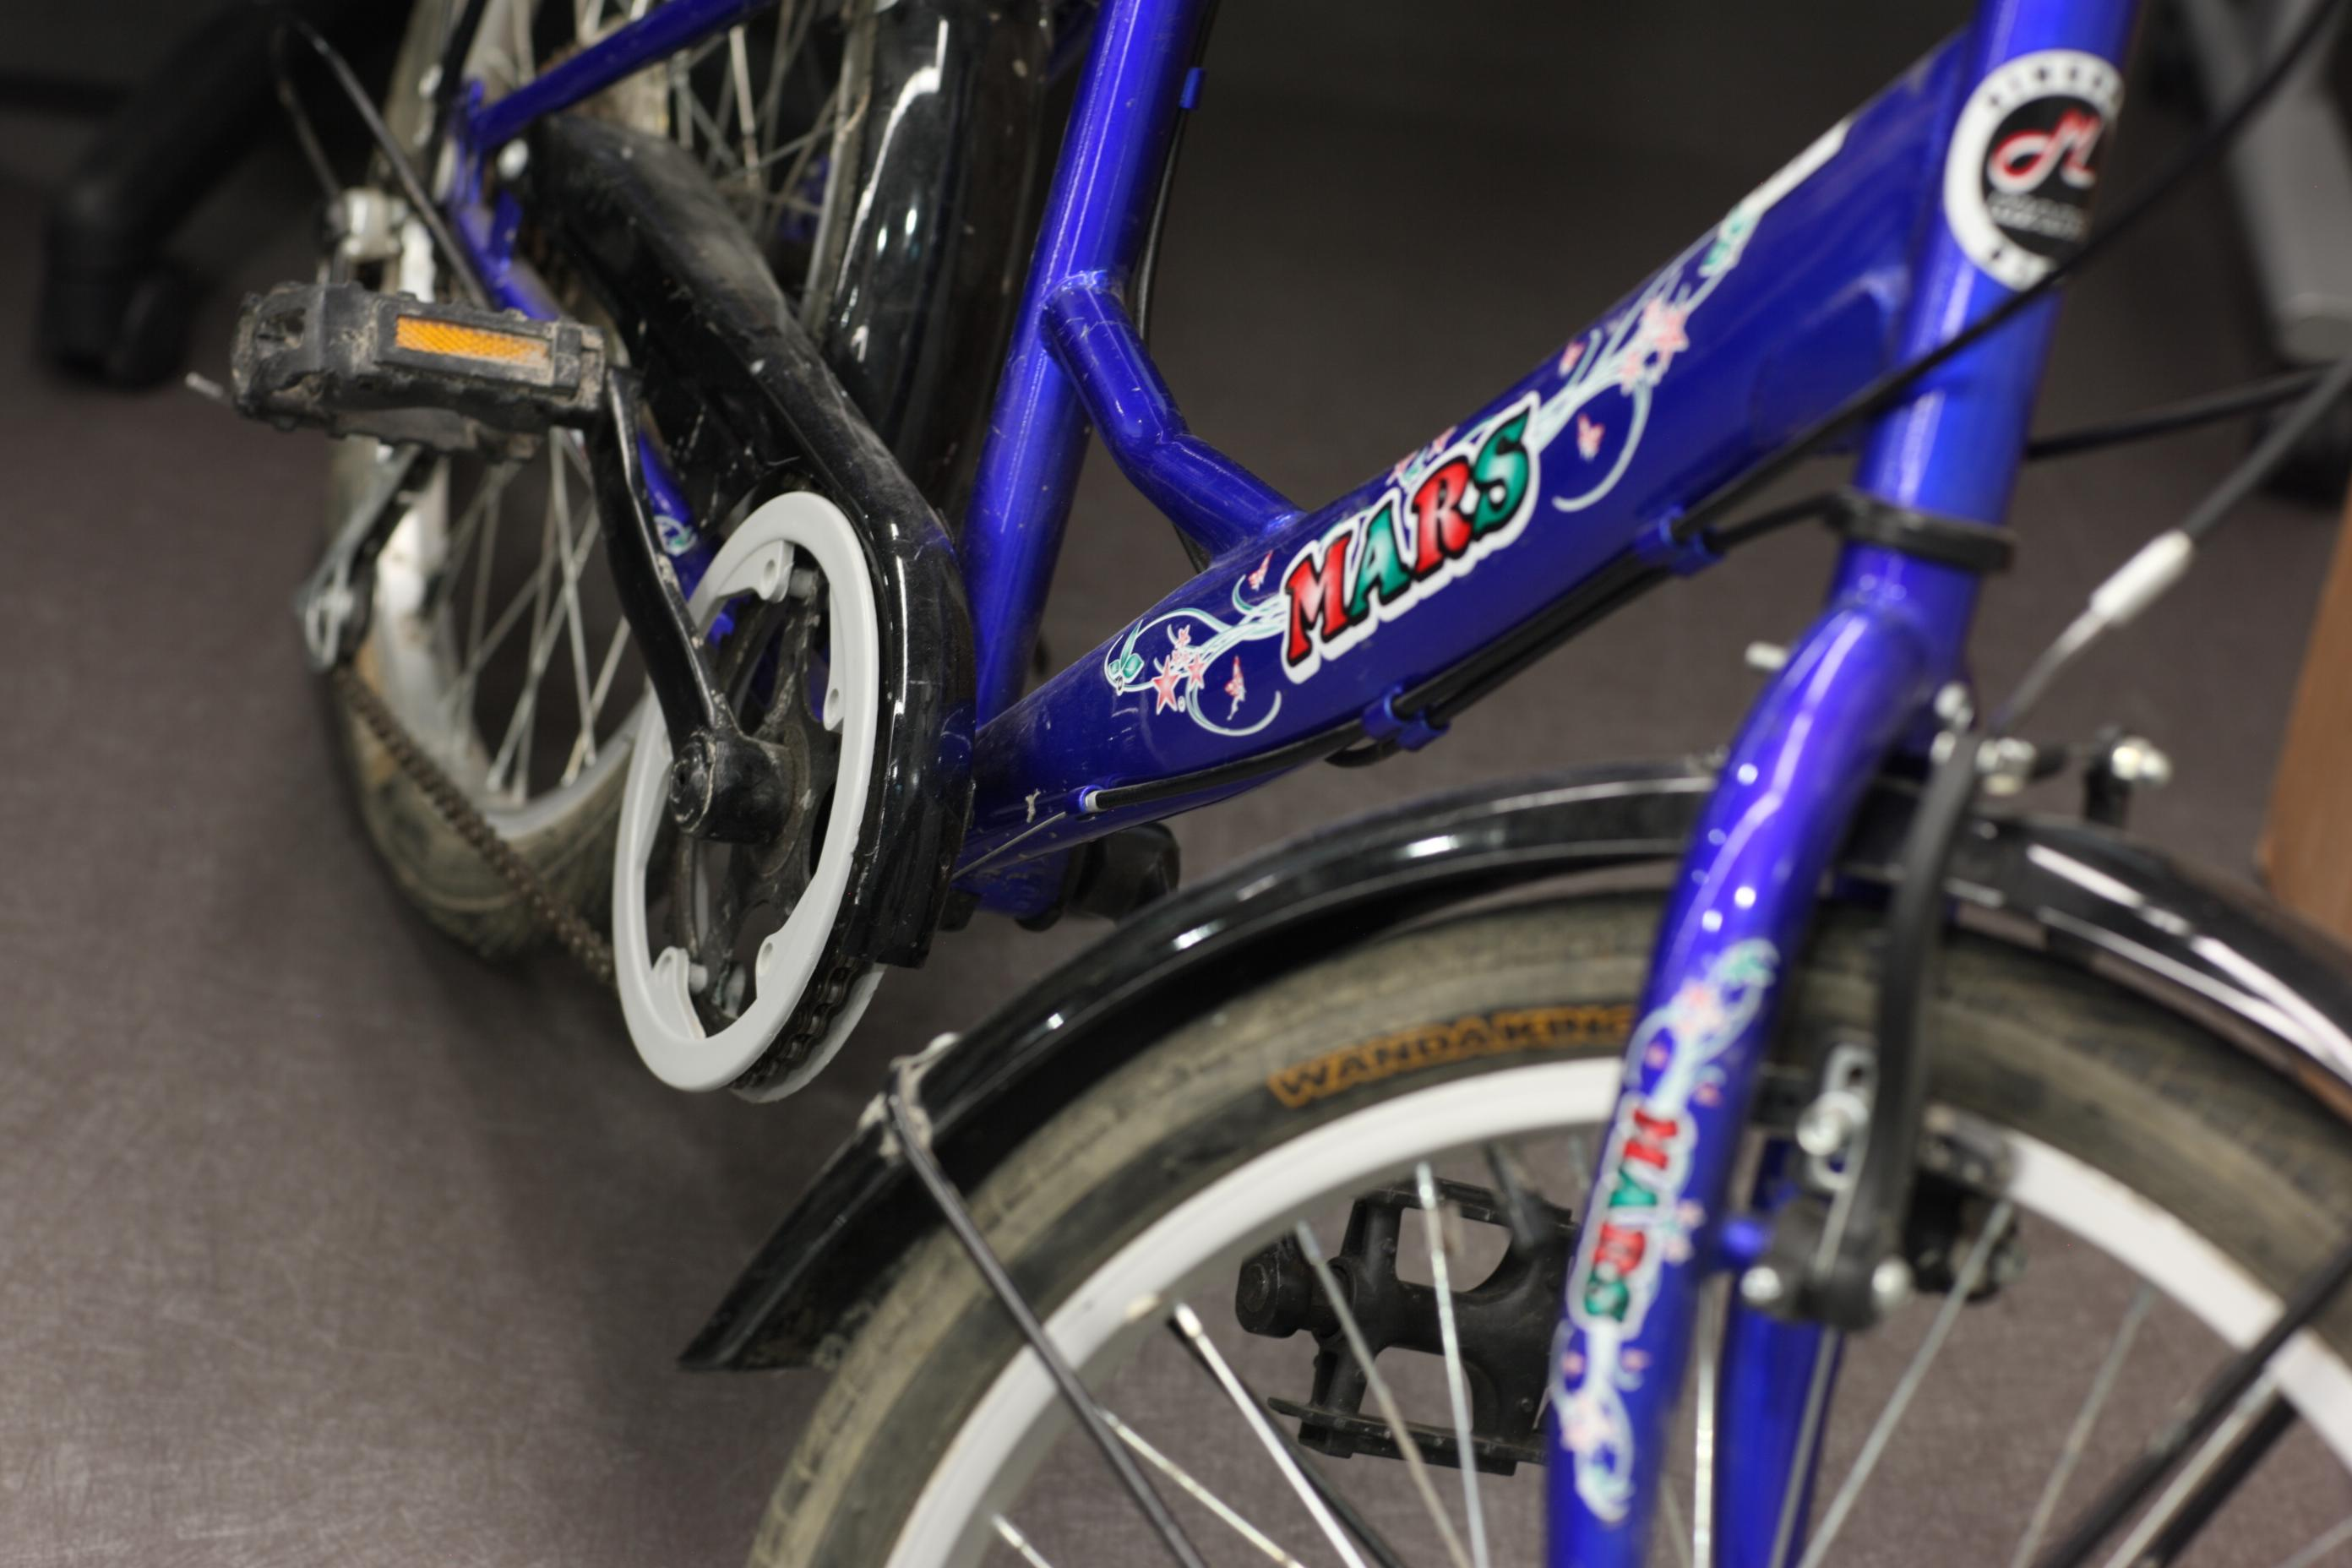
\includegraphics[width=1\textwidth]{images/dataset/Canon5D2_5_160_6400_bicycle_mean.JPG}
    \end{subfigure}
    \hfill
    \begin{subfigure}[t]{0.32\textwidth}
        \centering
        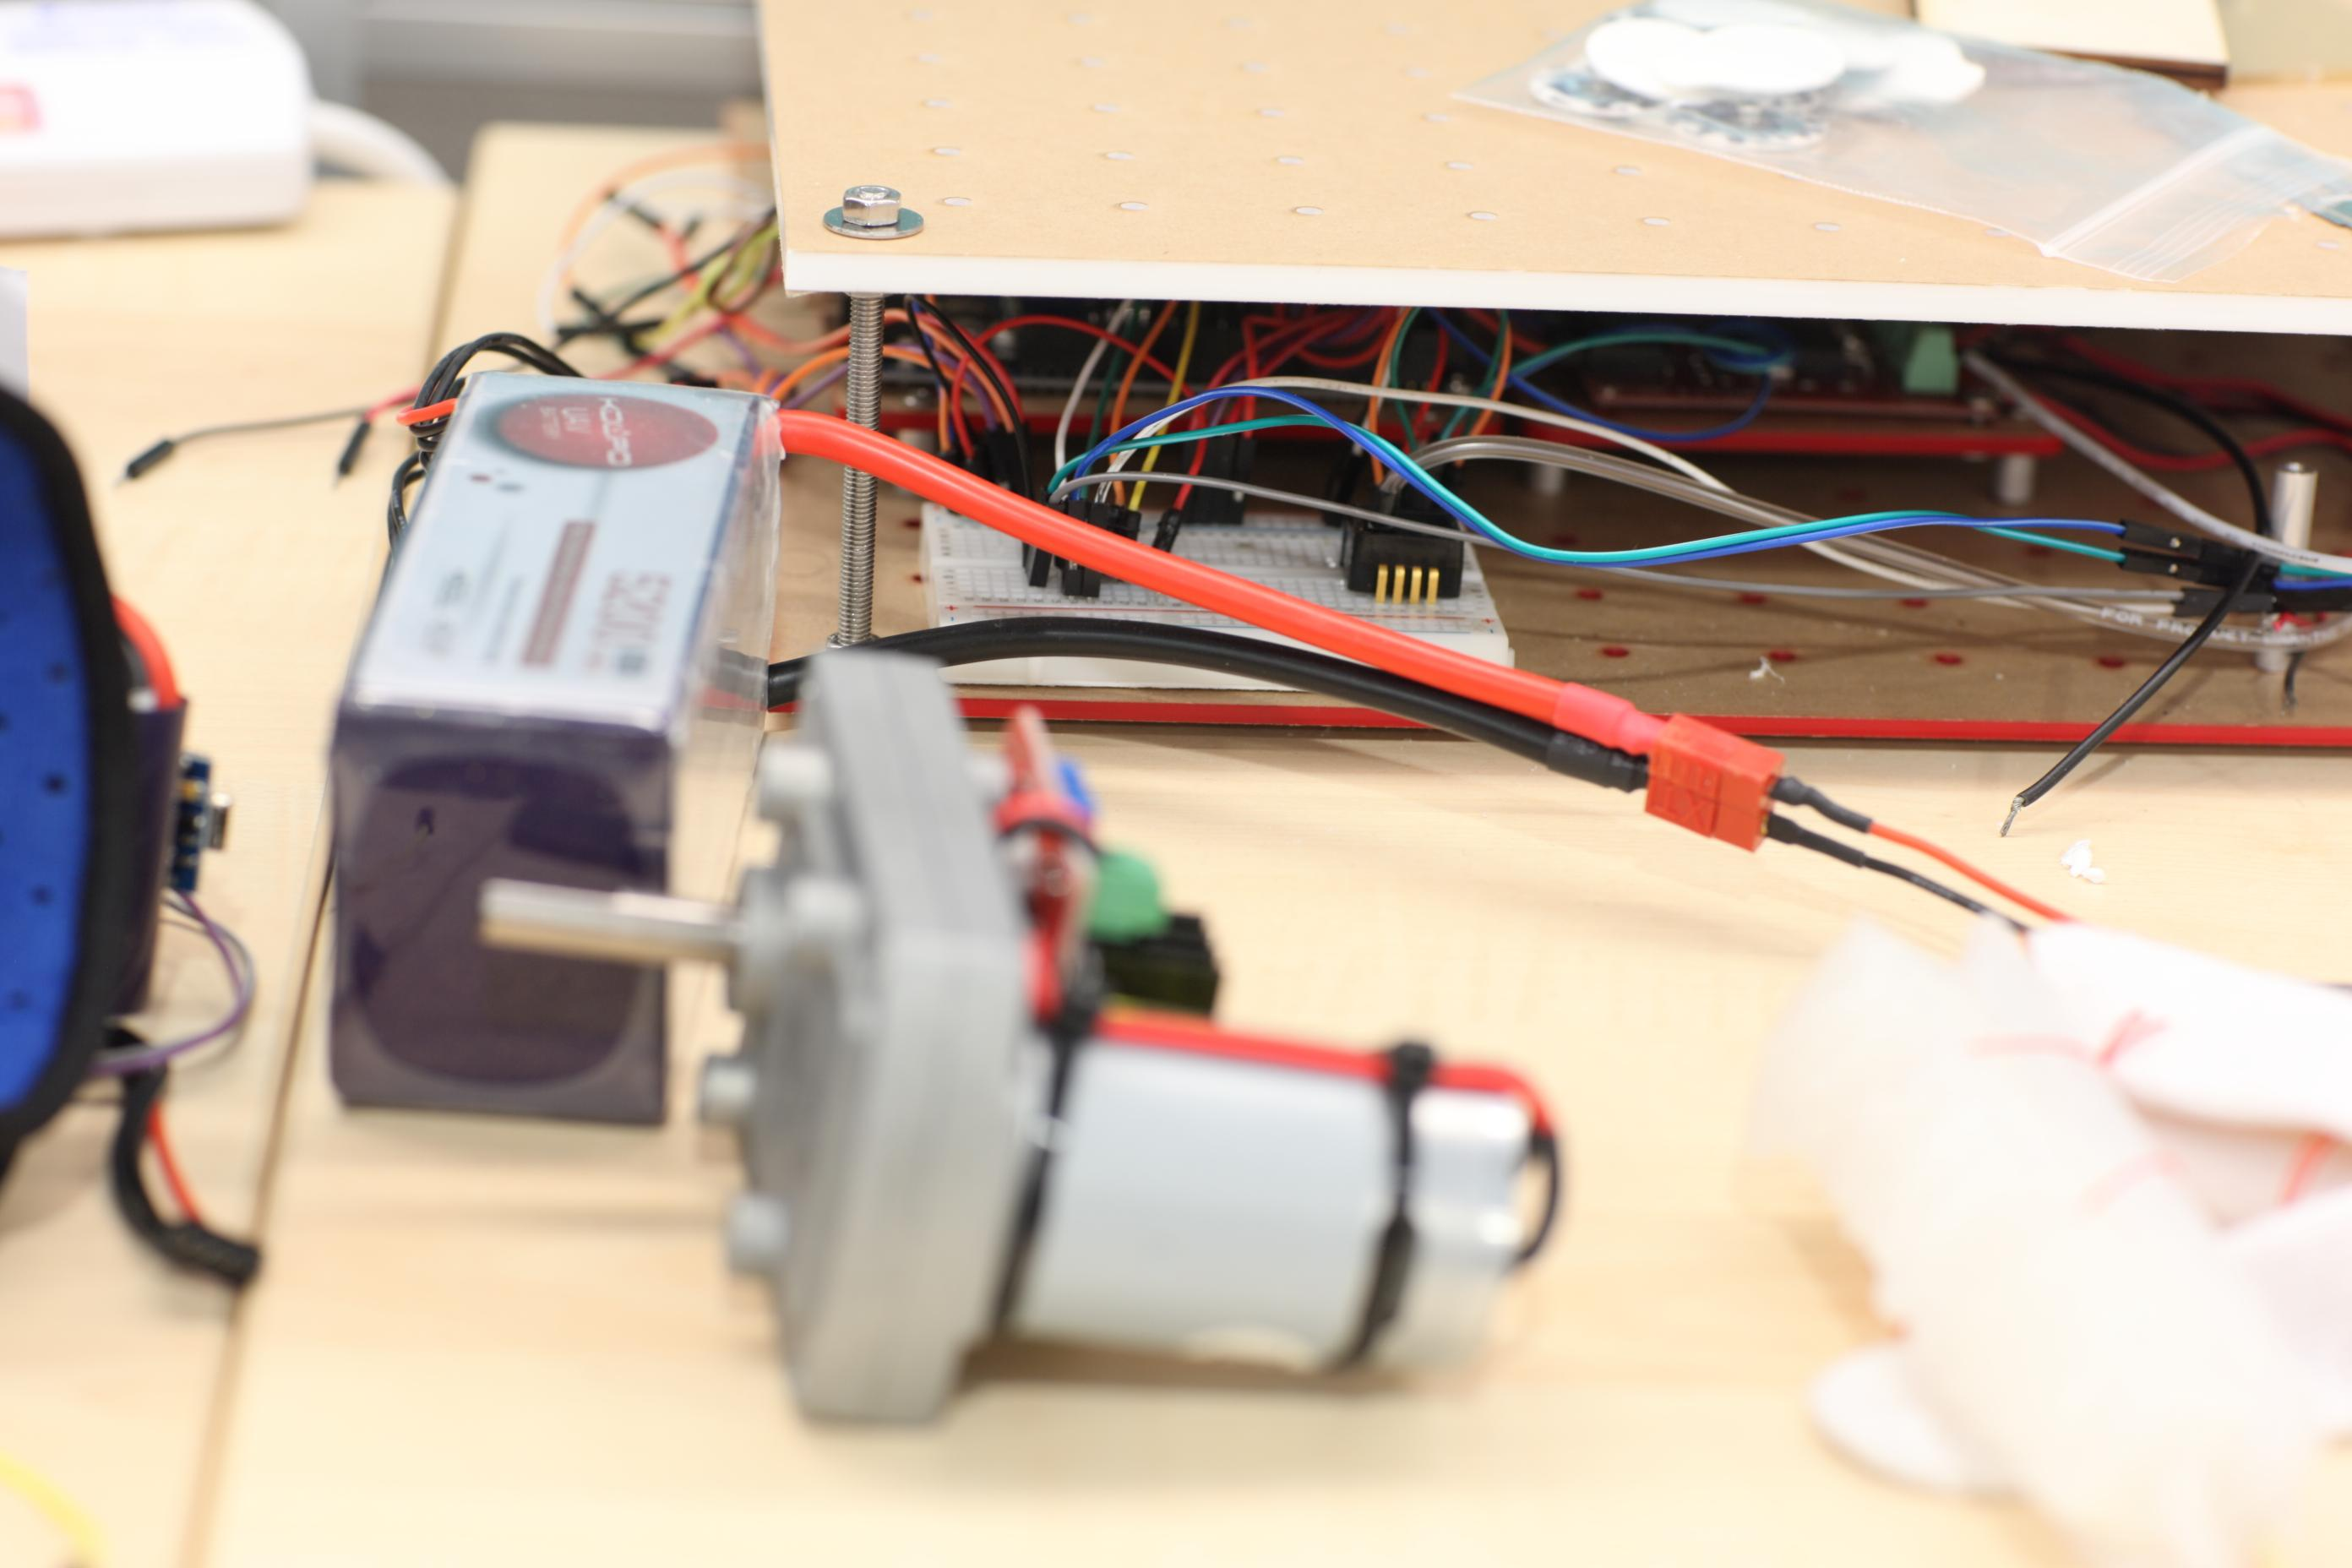
\includegraphics[width=1\textwidth]{images/dataset/Canon5D2_5_160_6400_circuit_mean.JPG}
    \end{subfigure}
    \hfill
    \begin{subfigure}[t]{0.32\textwidth}
        \centering
        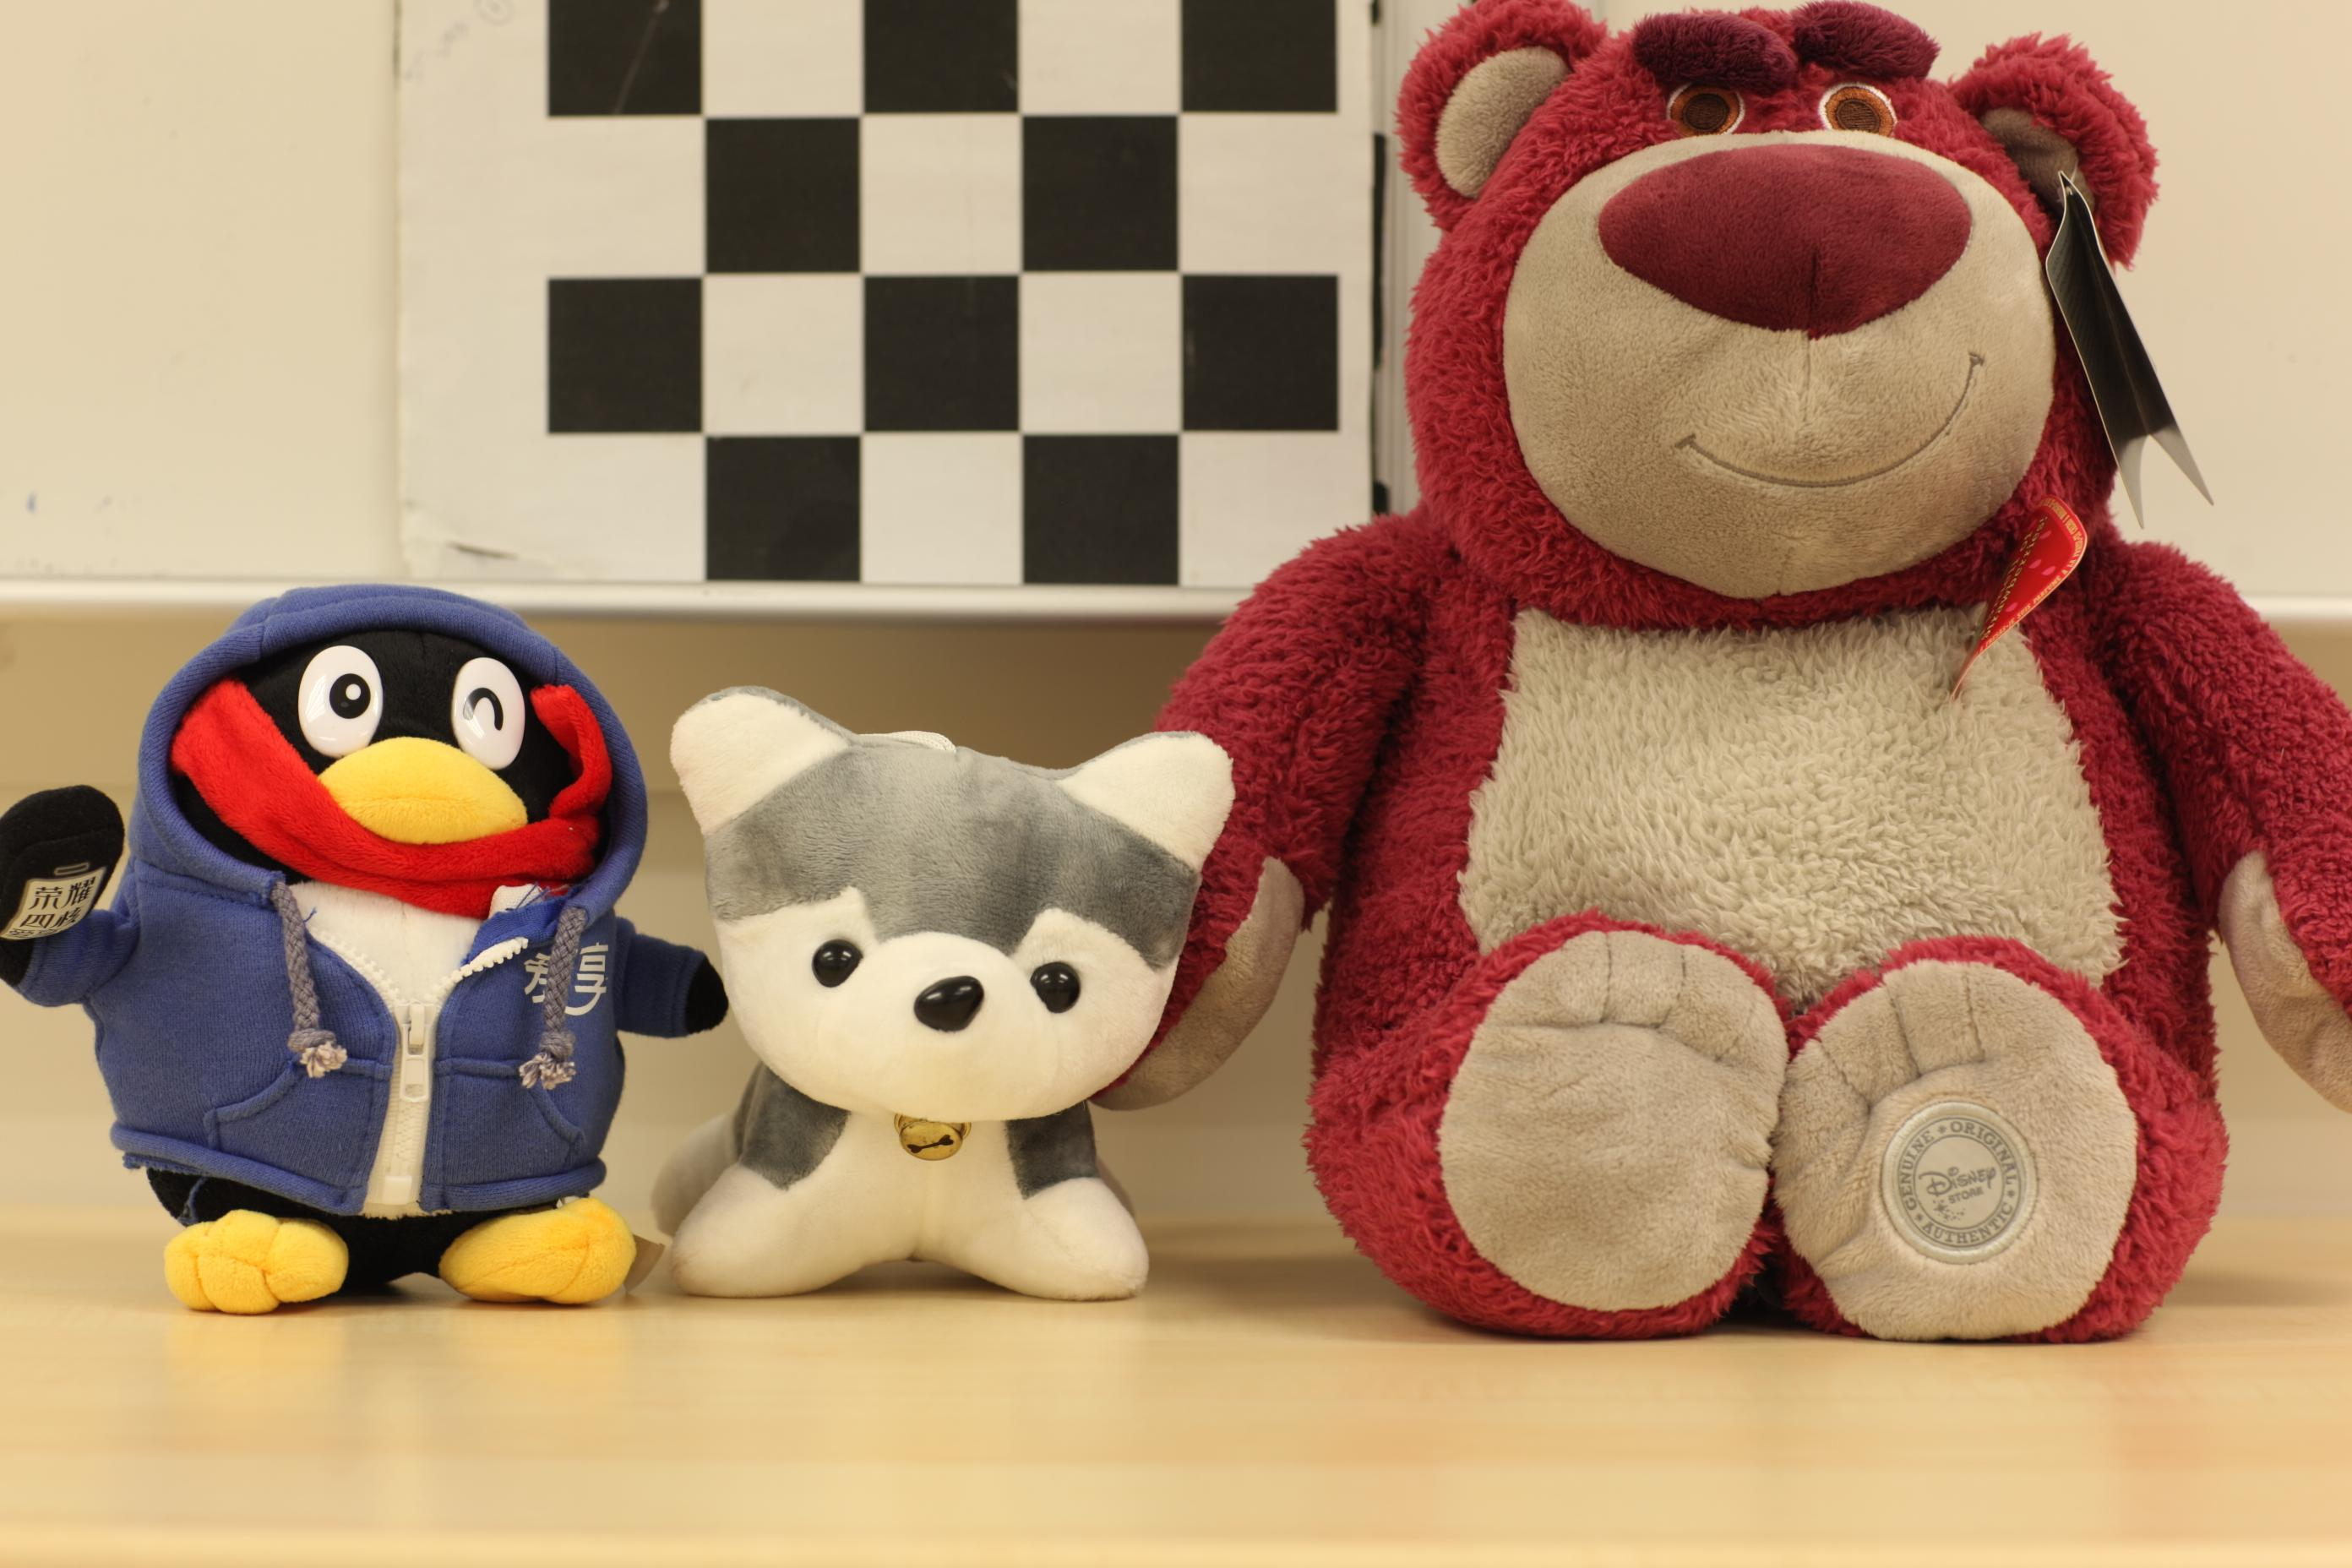
\includegraphics[width=1\textwidth]{images/dataset/Canon5D2_5_200_3200_toy_mean.JPG}
    \end{subfigure}
    \hfill
    \begin{subfigure}[t]{0.32\textwidth}
        \centering
        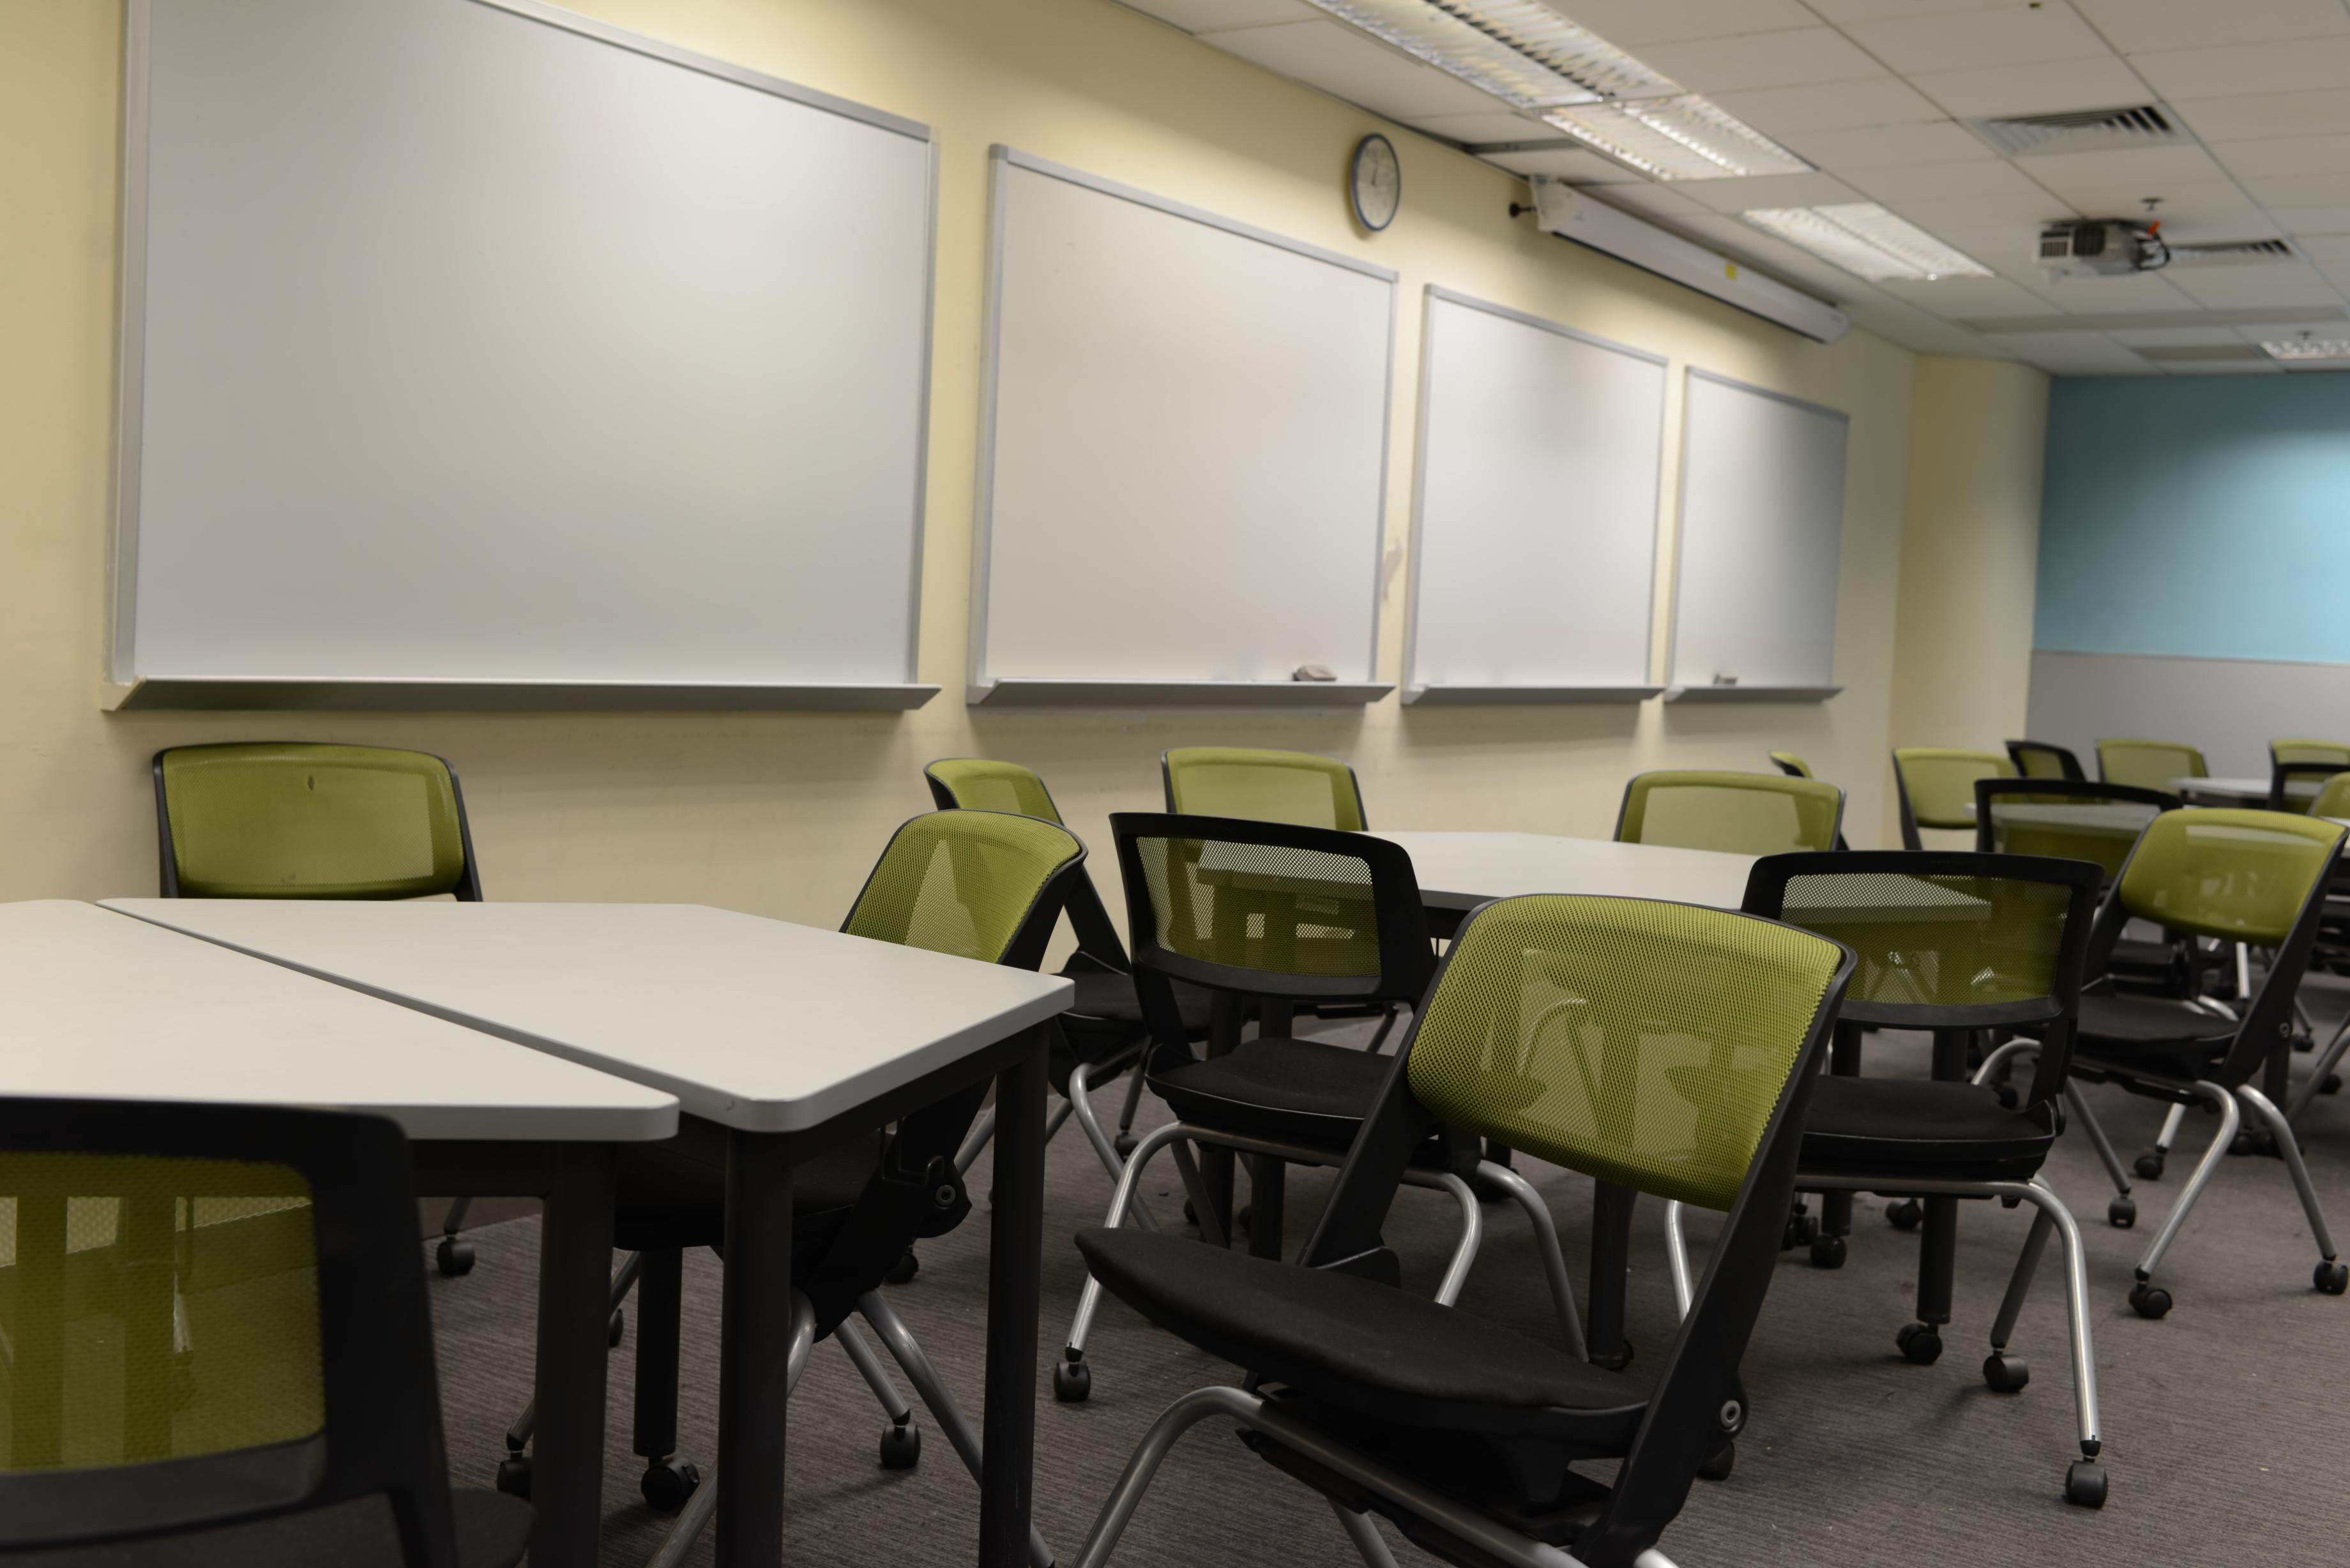
\includegraphics[width=1\textwidth]{images/dataset/NikonD800_4-5_160_1800_classroom_mean.JPG}
    \end{subfigure}
    \hfill
    \begin{subfigure}[t]{0.32\textwidth}
        \centering
        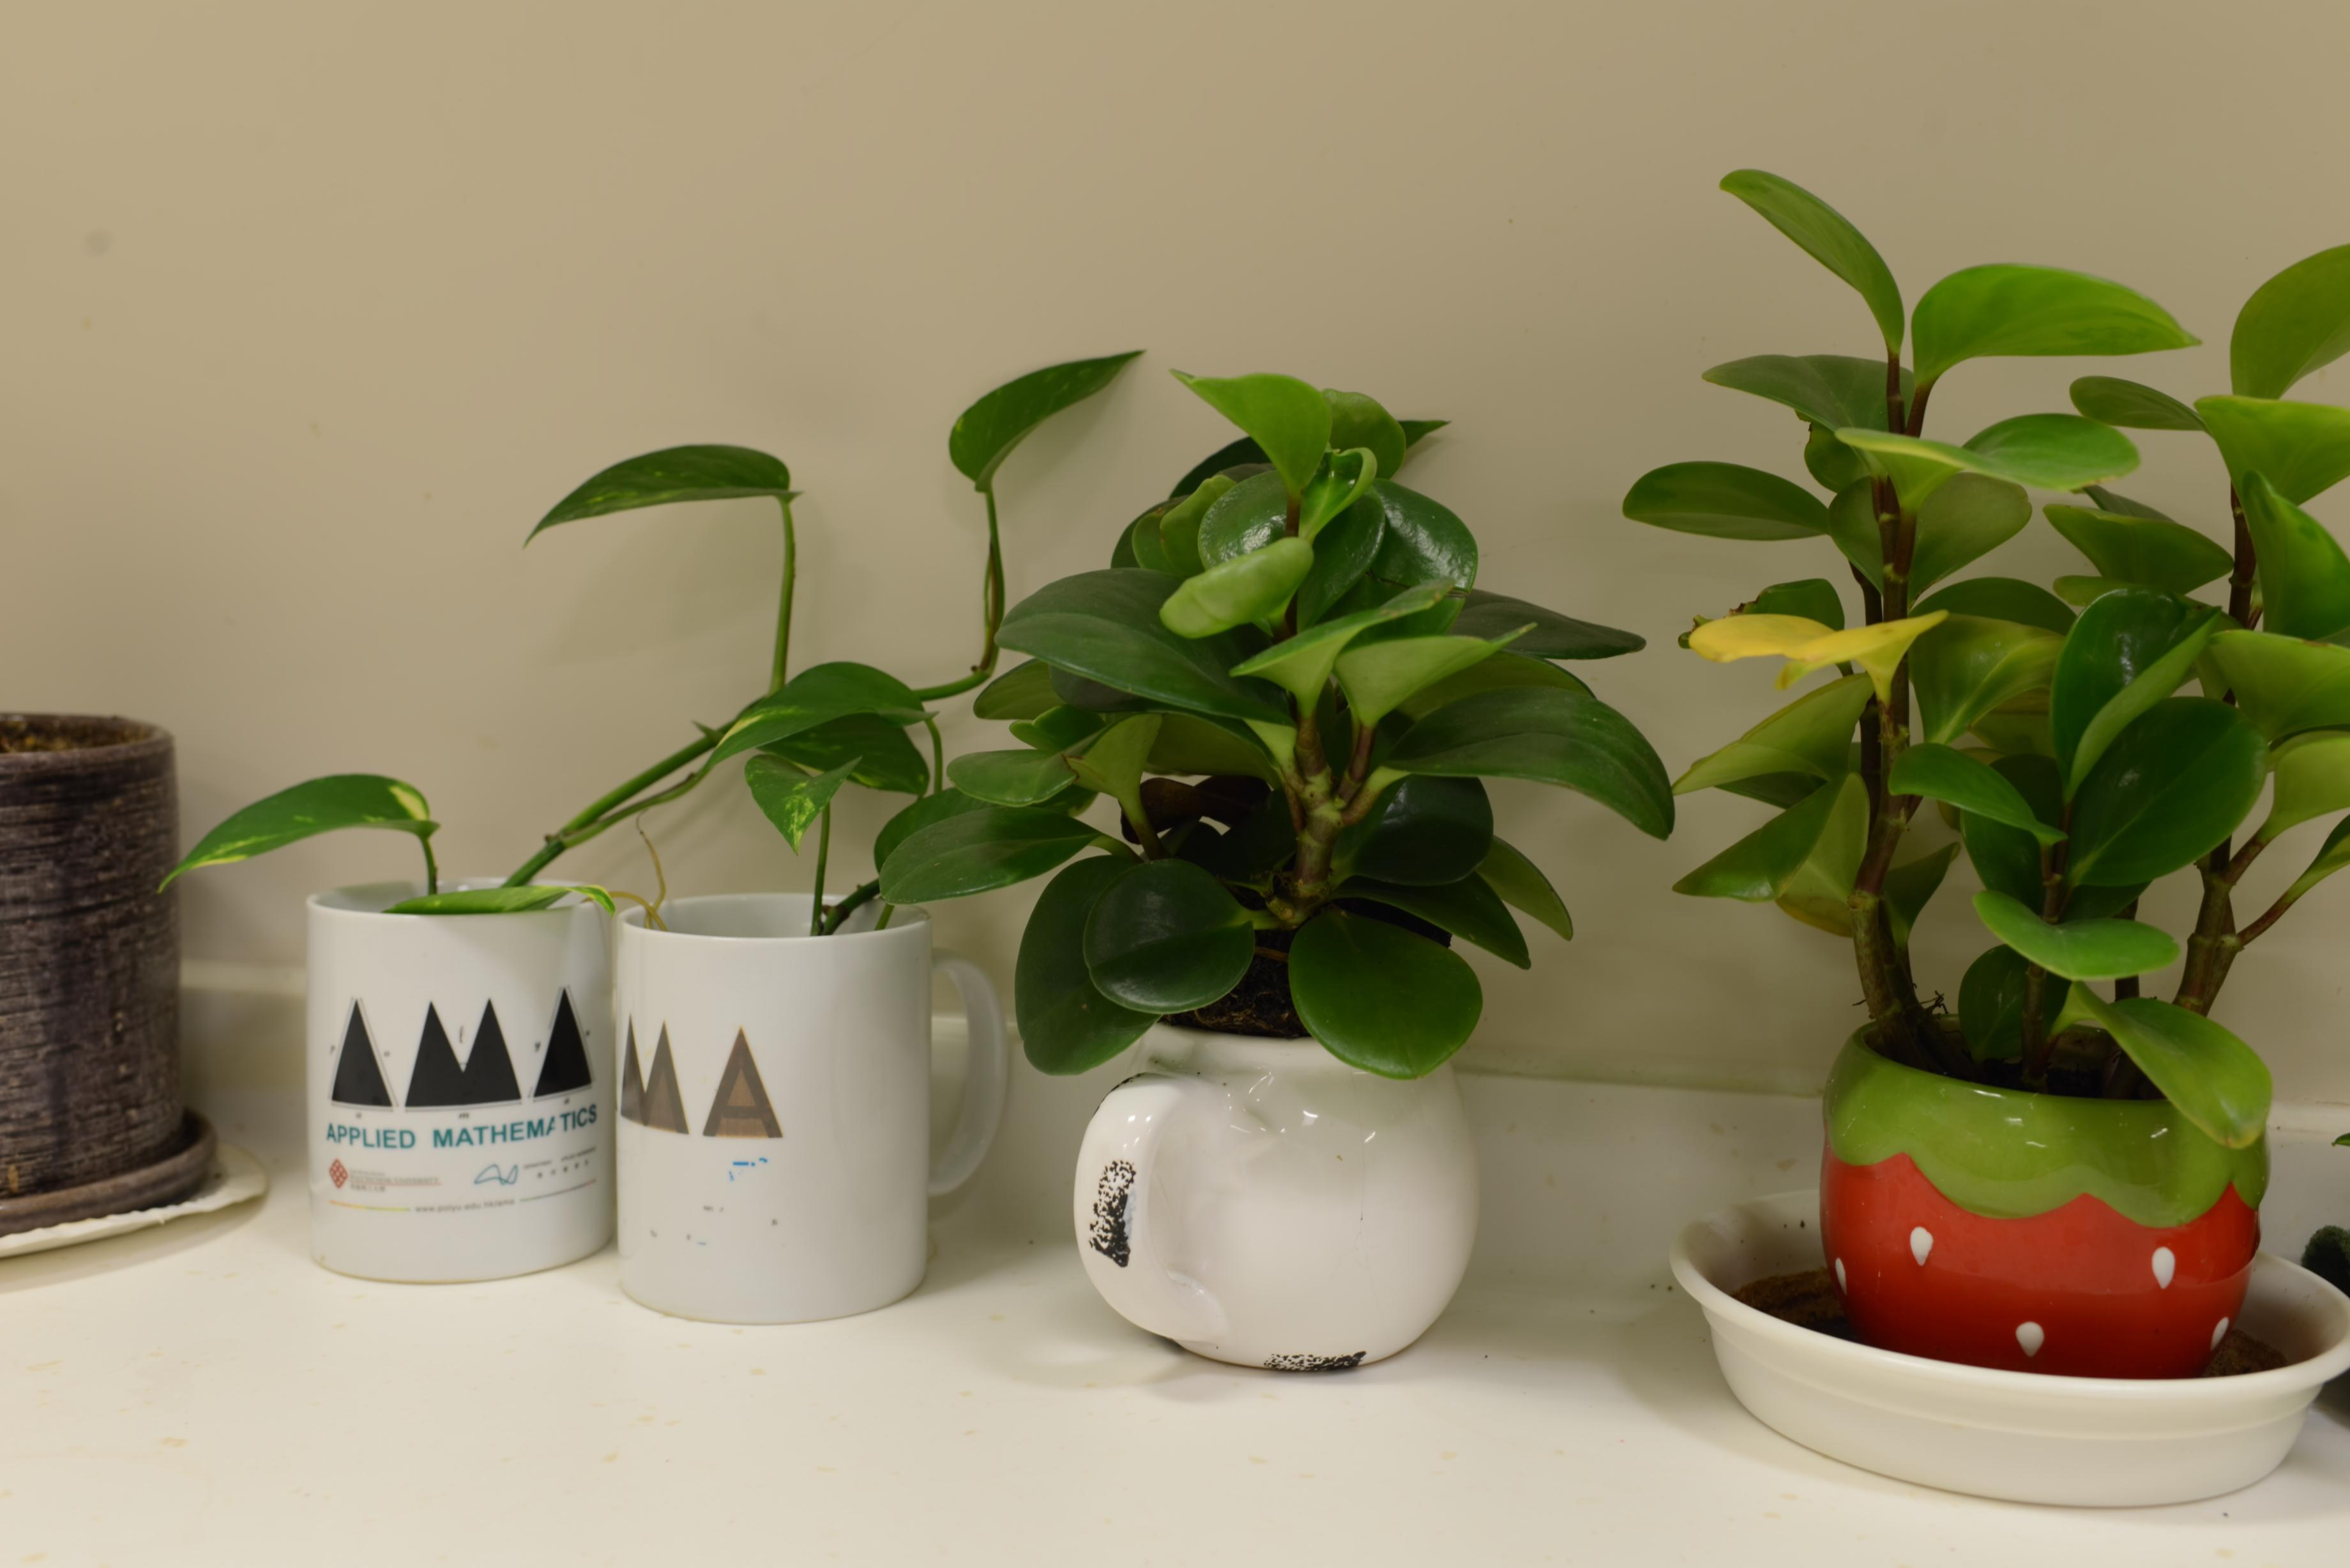
\includegraphics[width=1\textwidth]{images/dataset/NikonD800_6-3_125_5000_plant_mean.JPG}
    \end{subfigure}
    \hfill
    \begin{subfigure}[t]{0.32\textwidth}
        \centering
        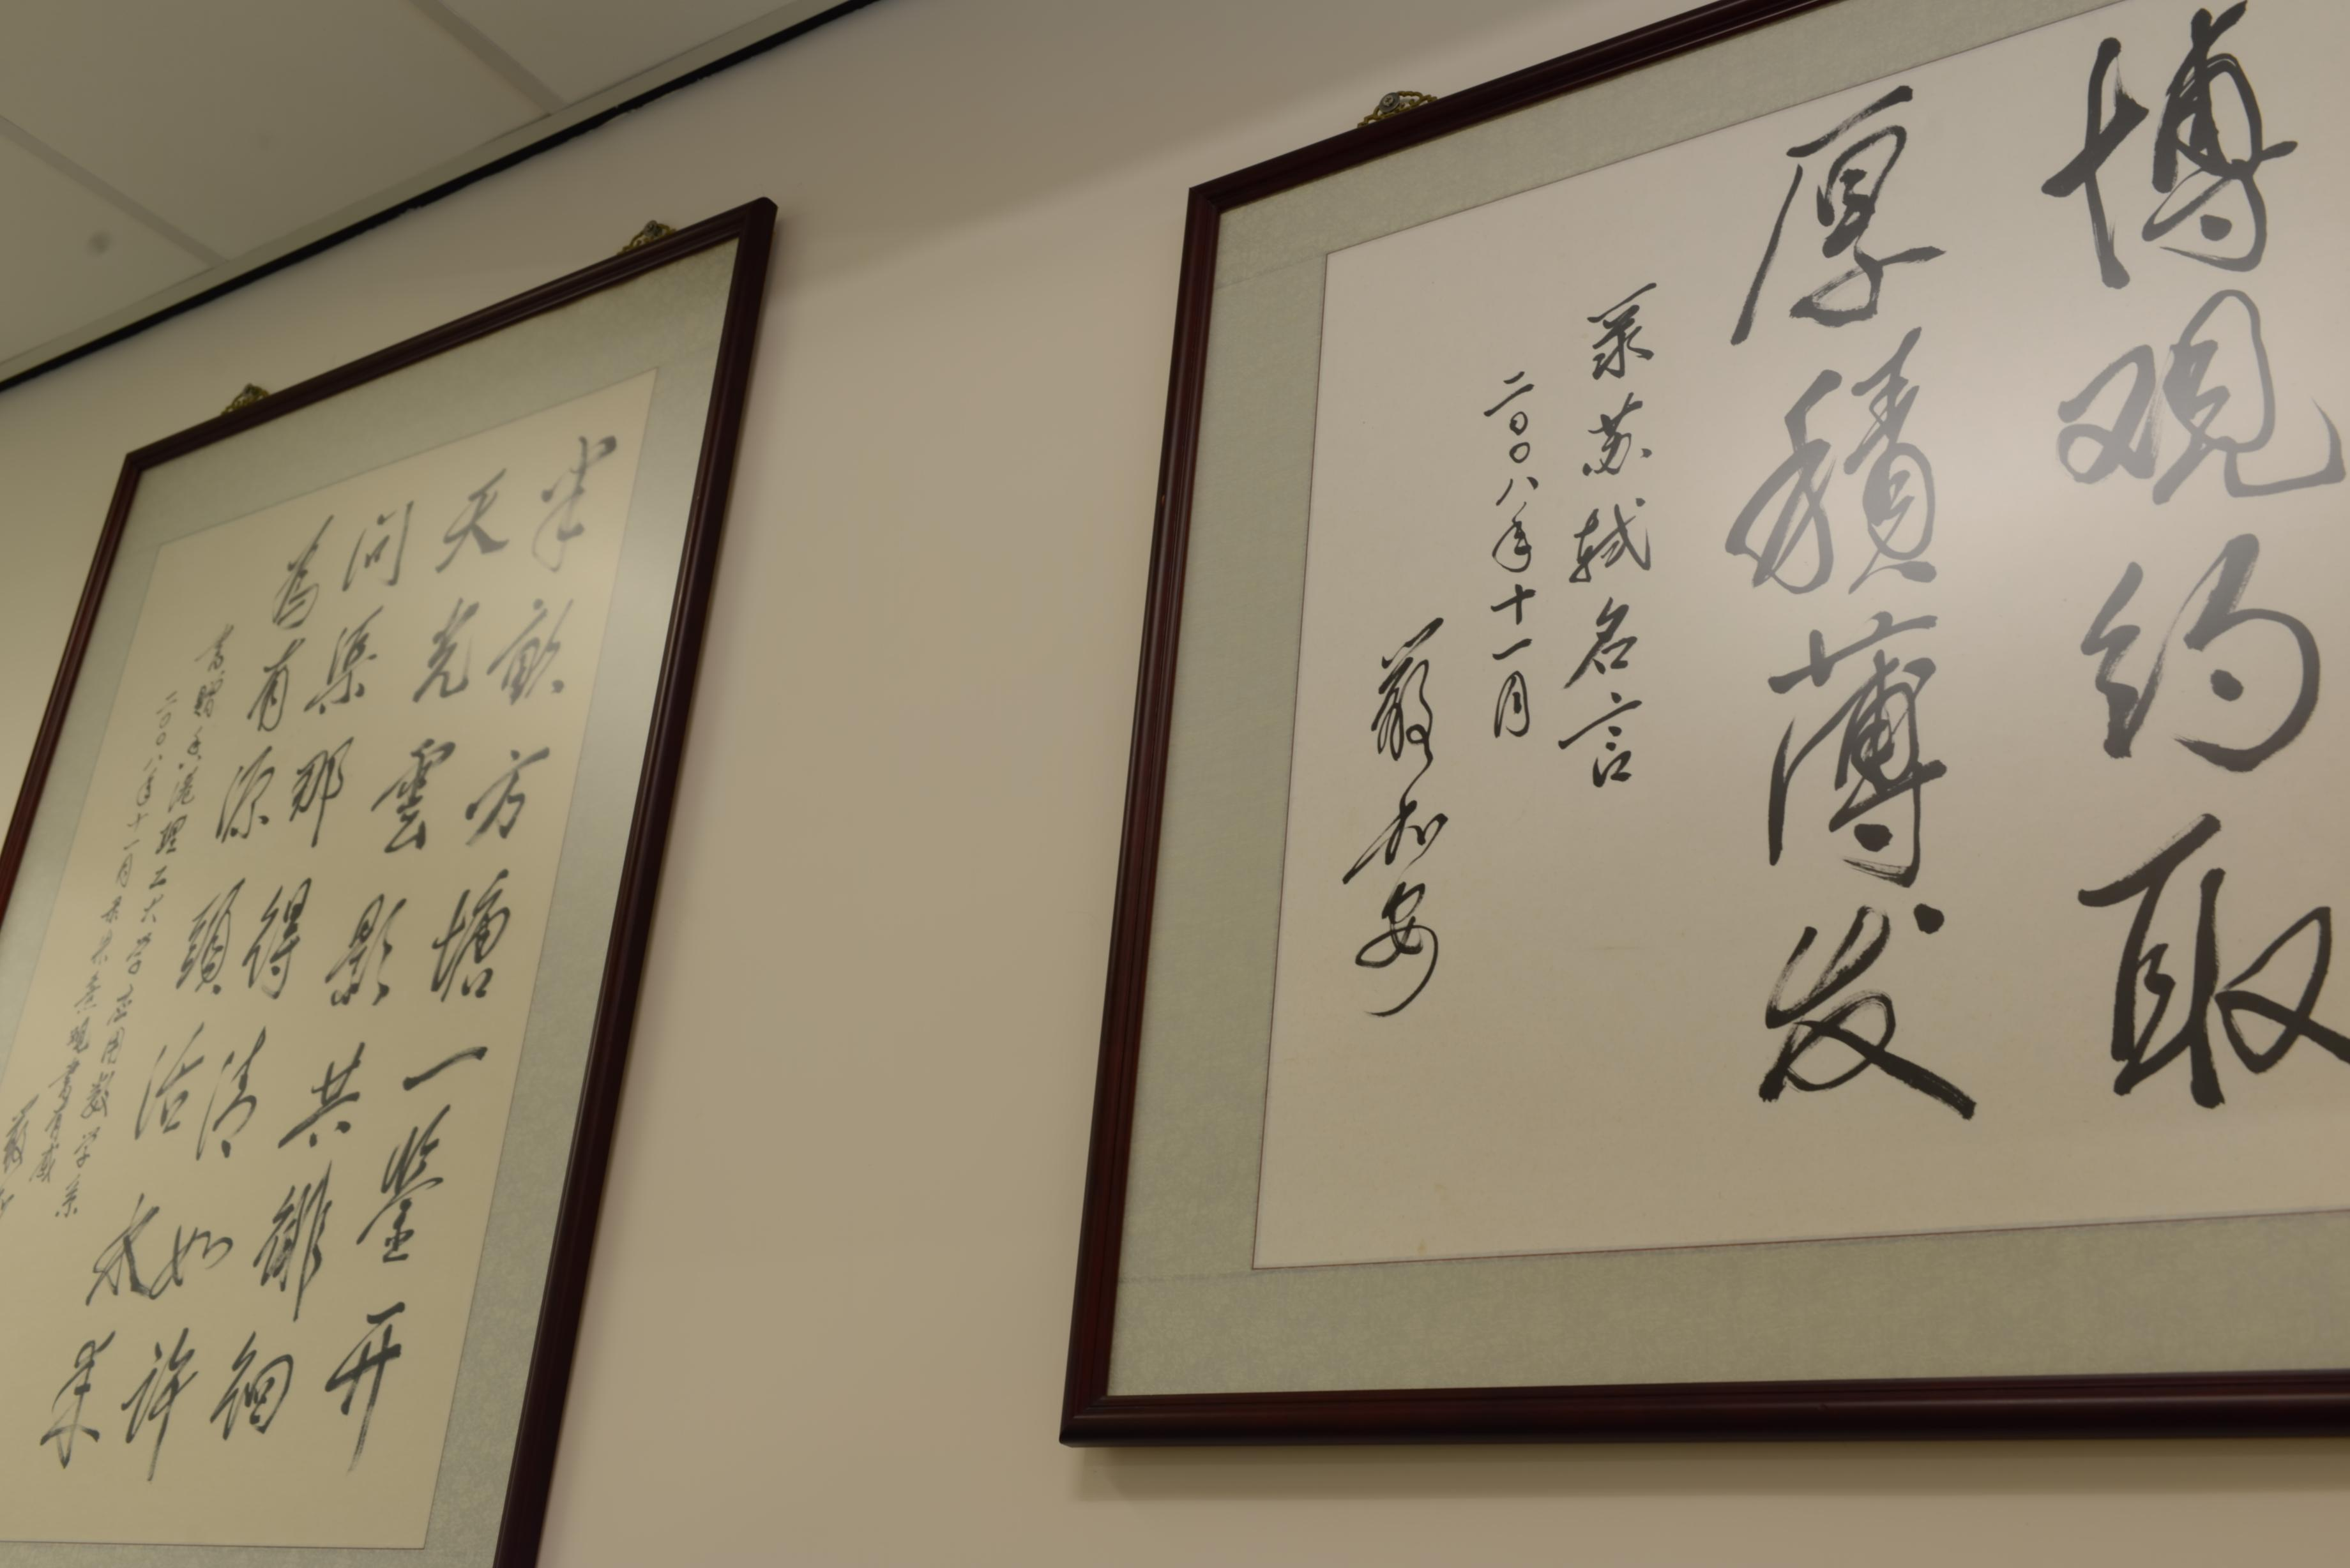
\includegraphics[width=1\textwidth]{images/dataset/NikonD800_8_125_6400_photo_mean.JPG}
    \end{subfigure}
    \hfill
    \begin{subfigure}[t]{0.32\textwidth}
        \centering
        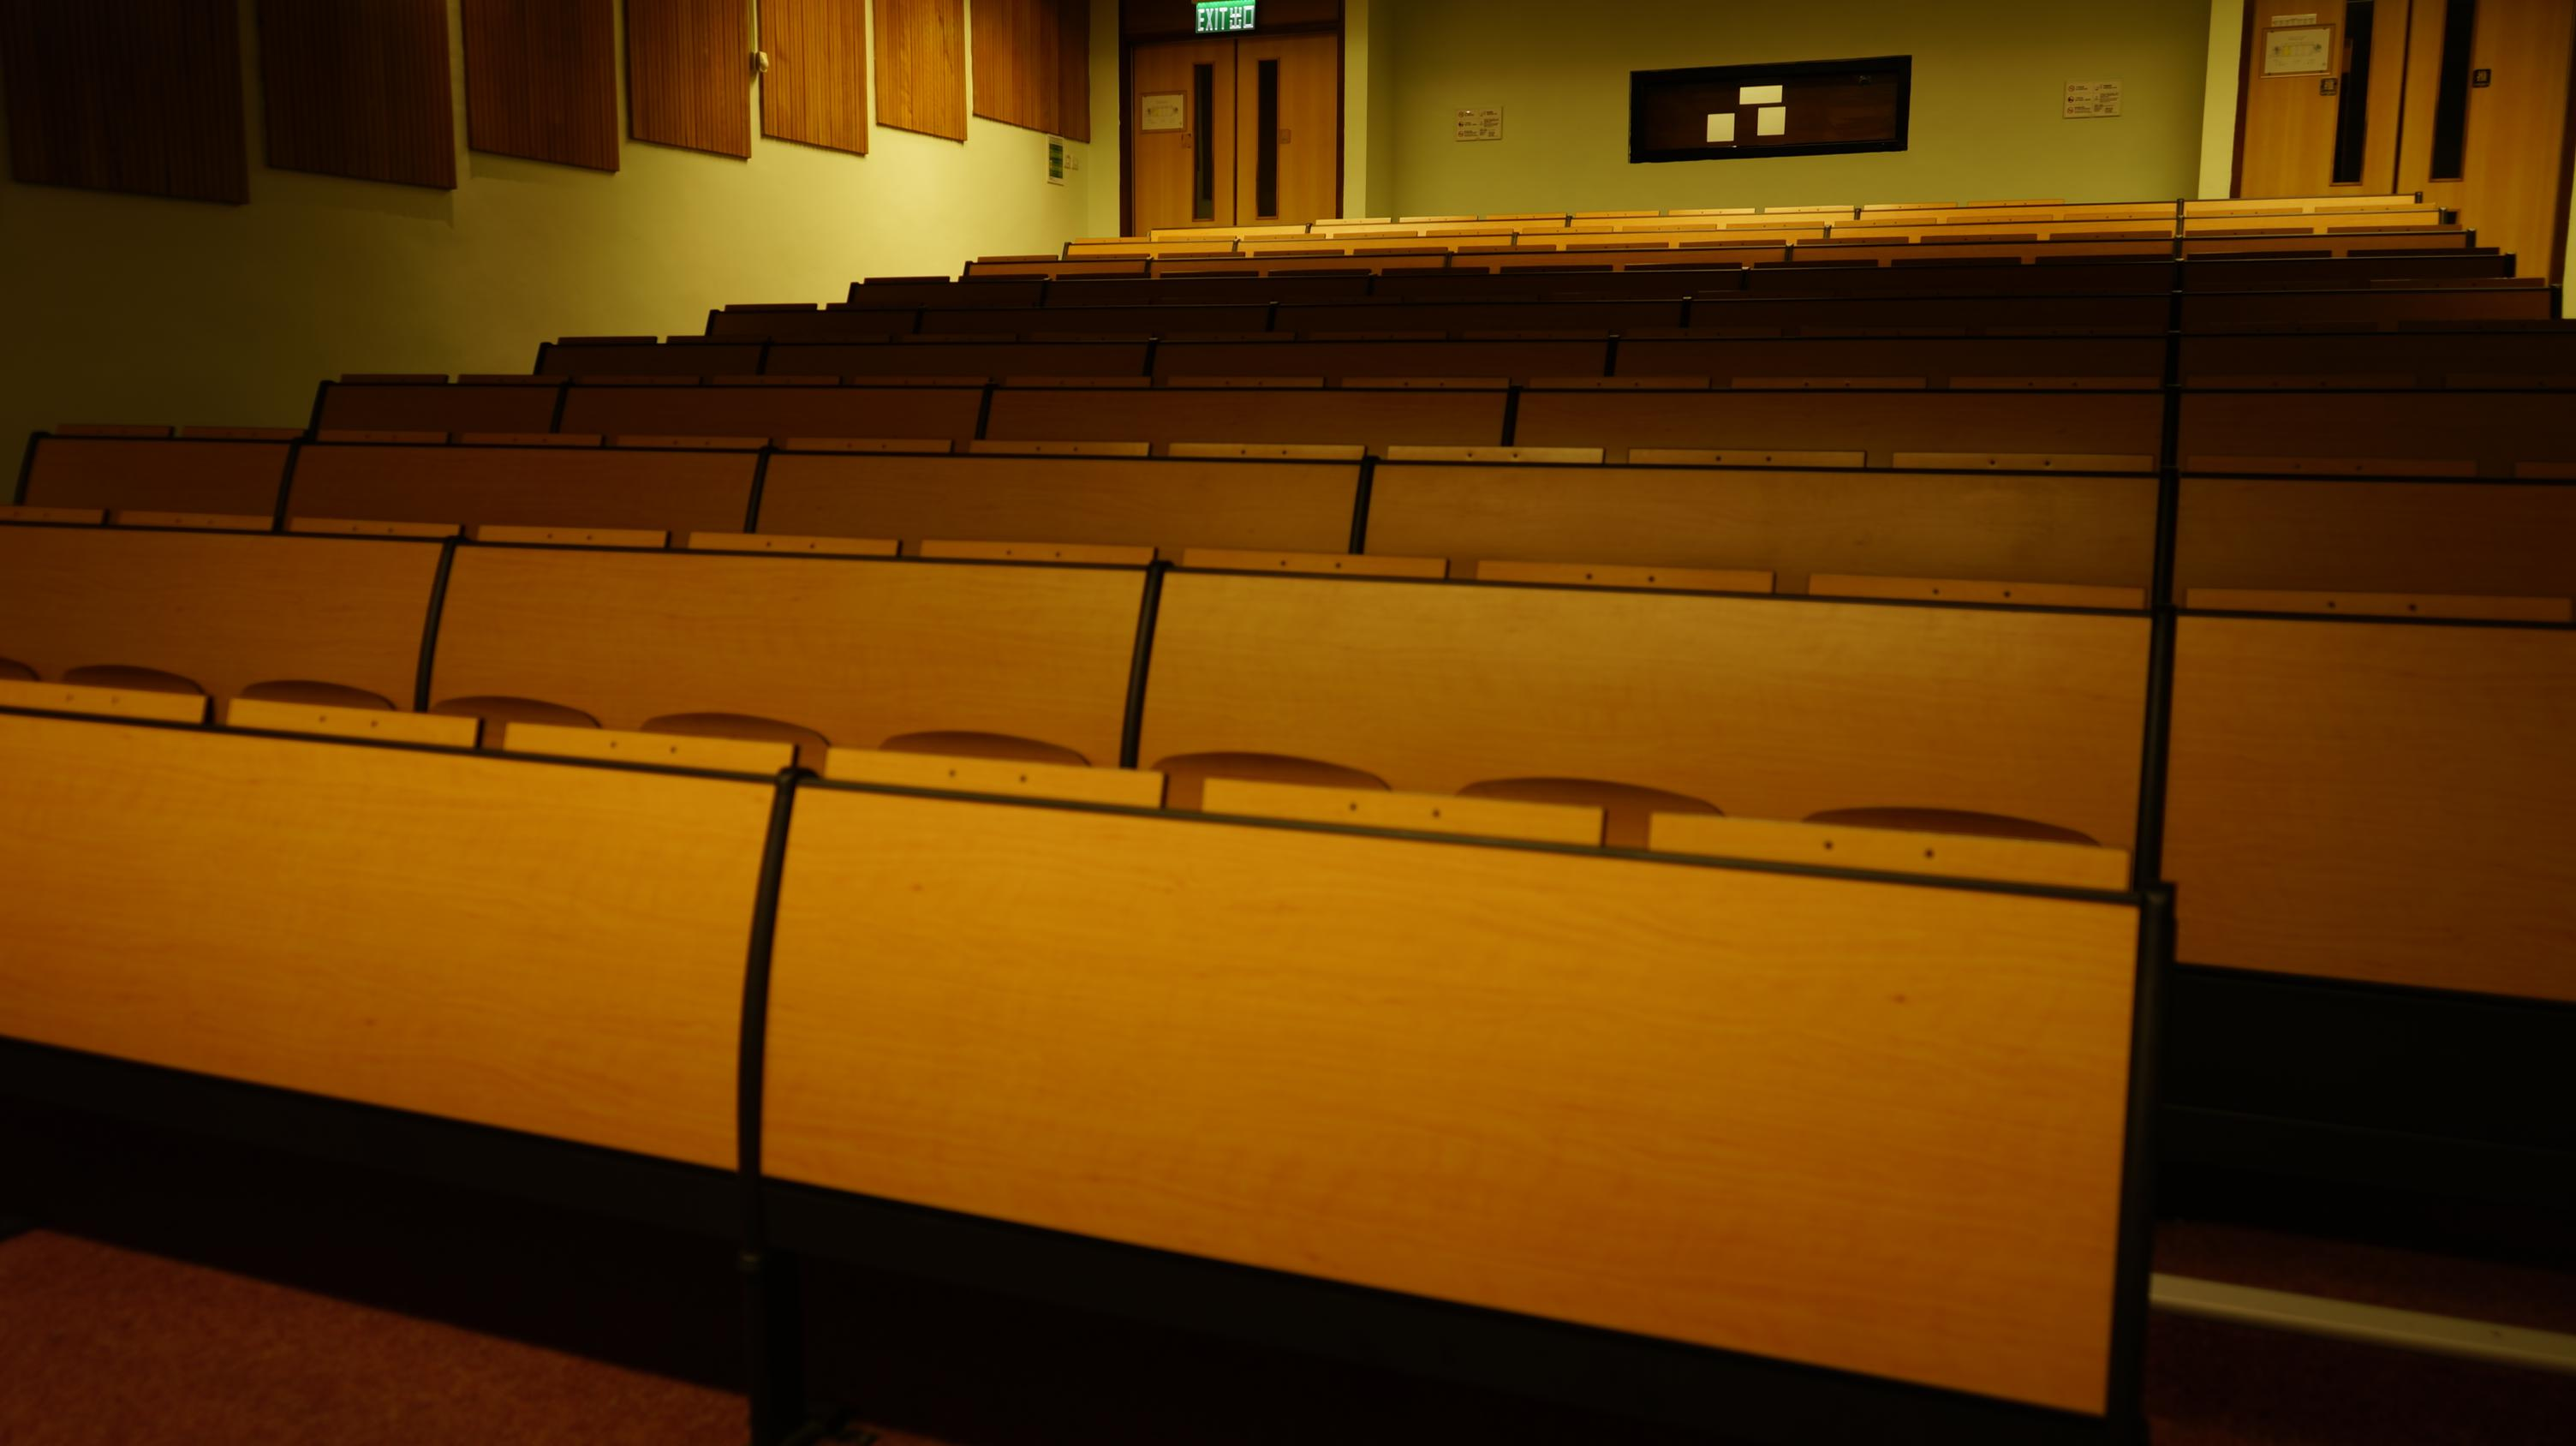
\includegraphics[width=1\textwidth]{images/dataset/Sony_3-5_200_1600_classroom_mean.JPG}
    \end{subfigure}
    \hfill
    \begin{subfigure}[t]{0.32\textwidth}
        \centering
        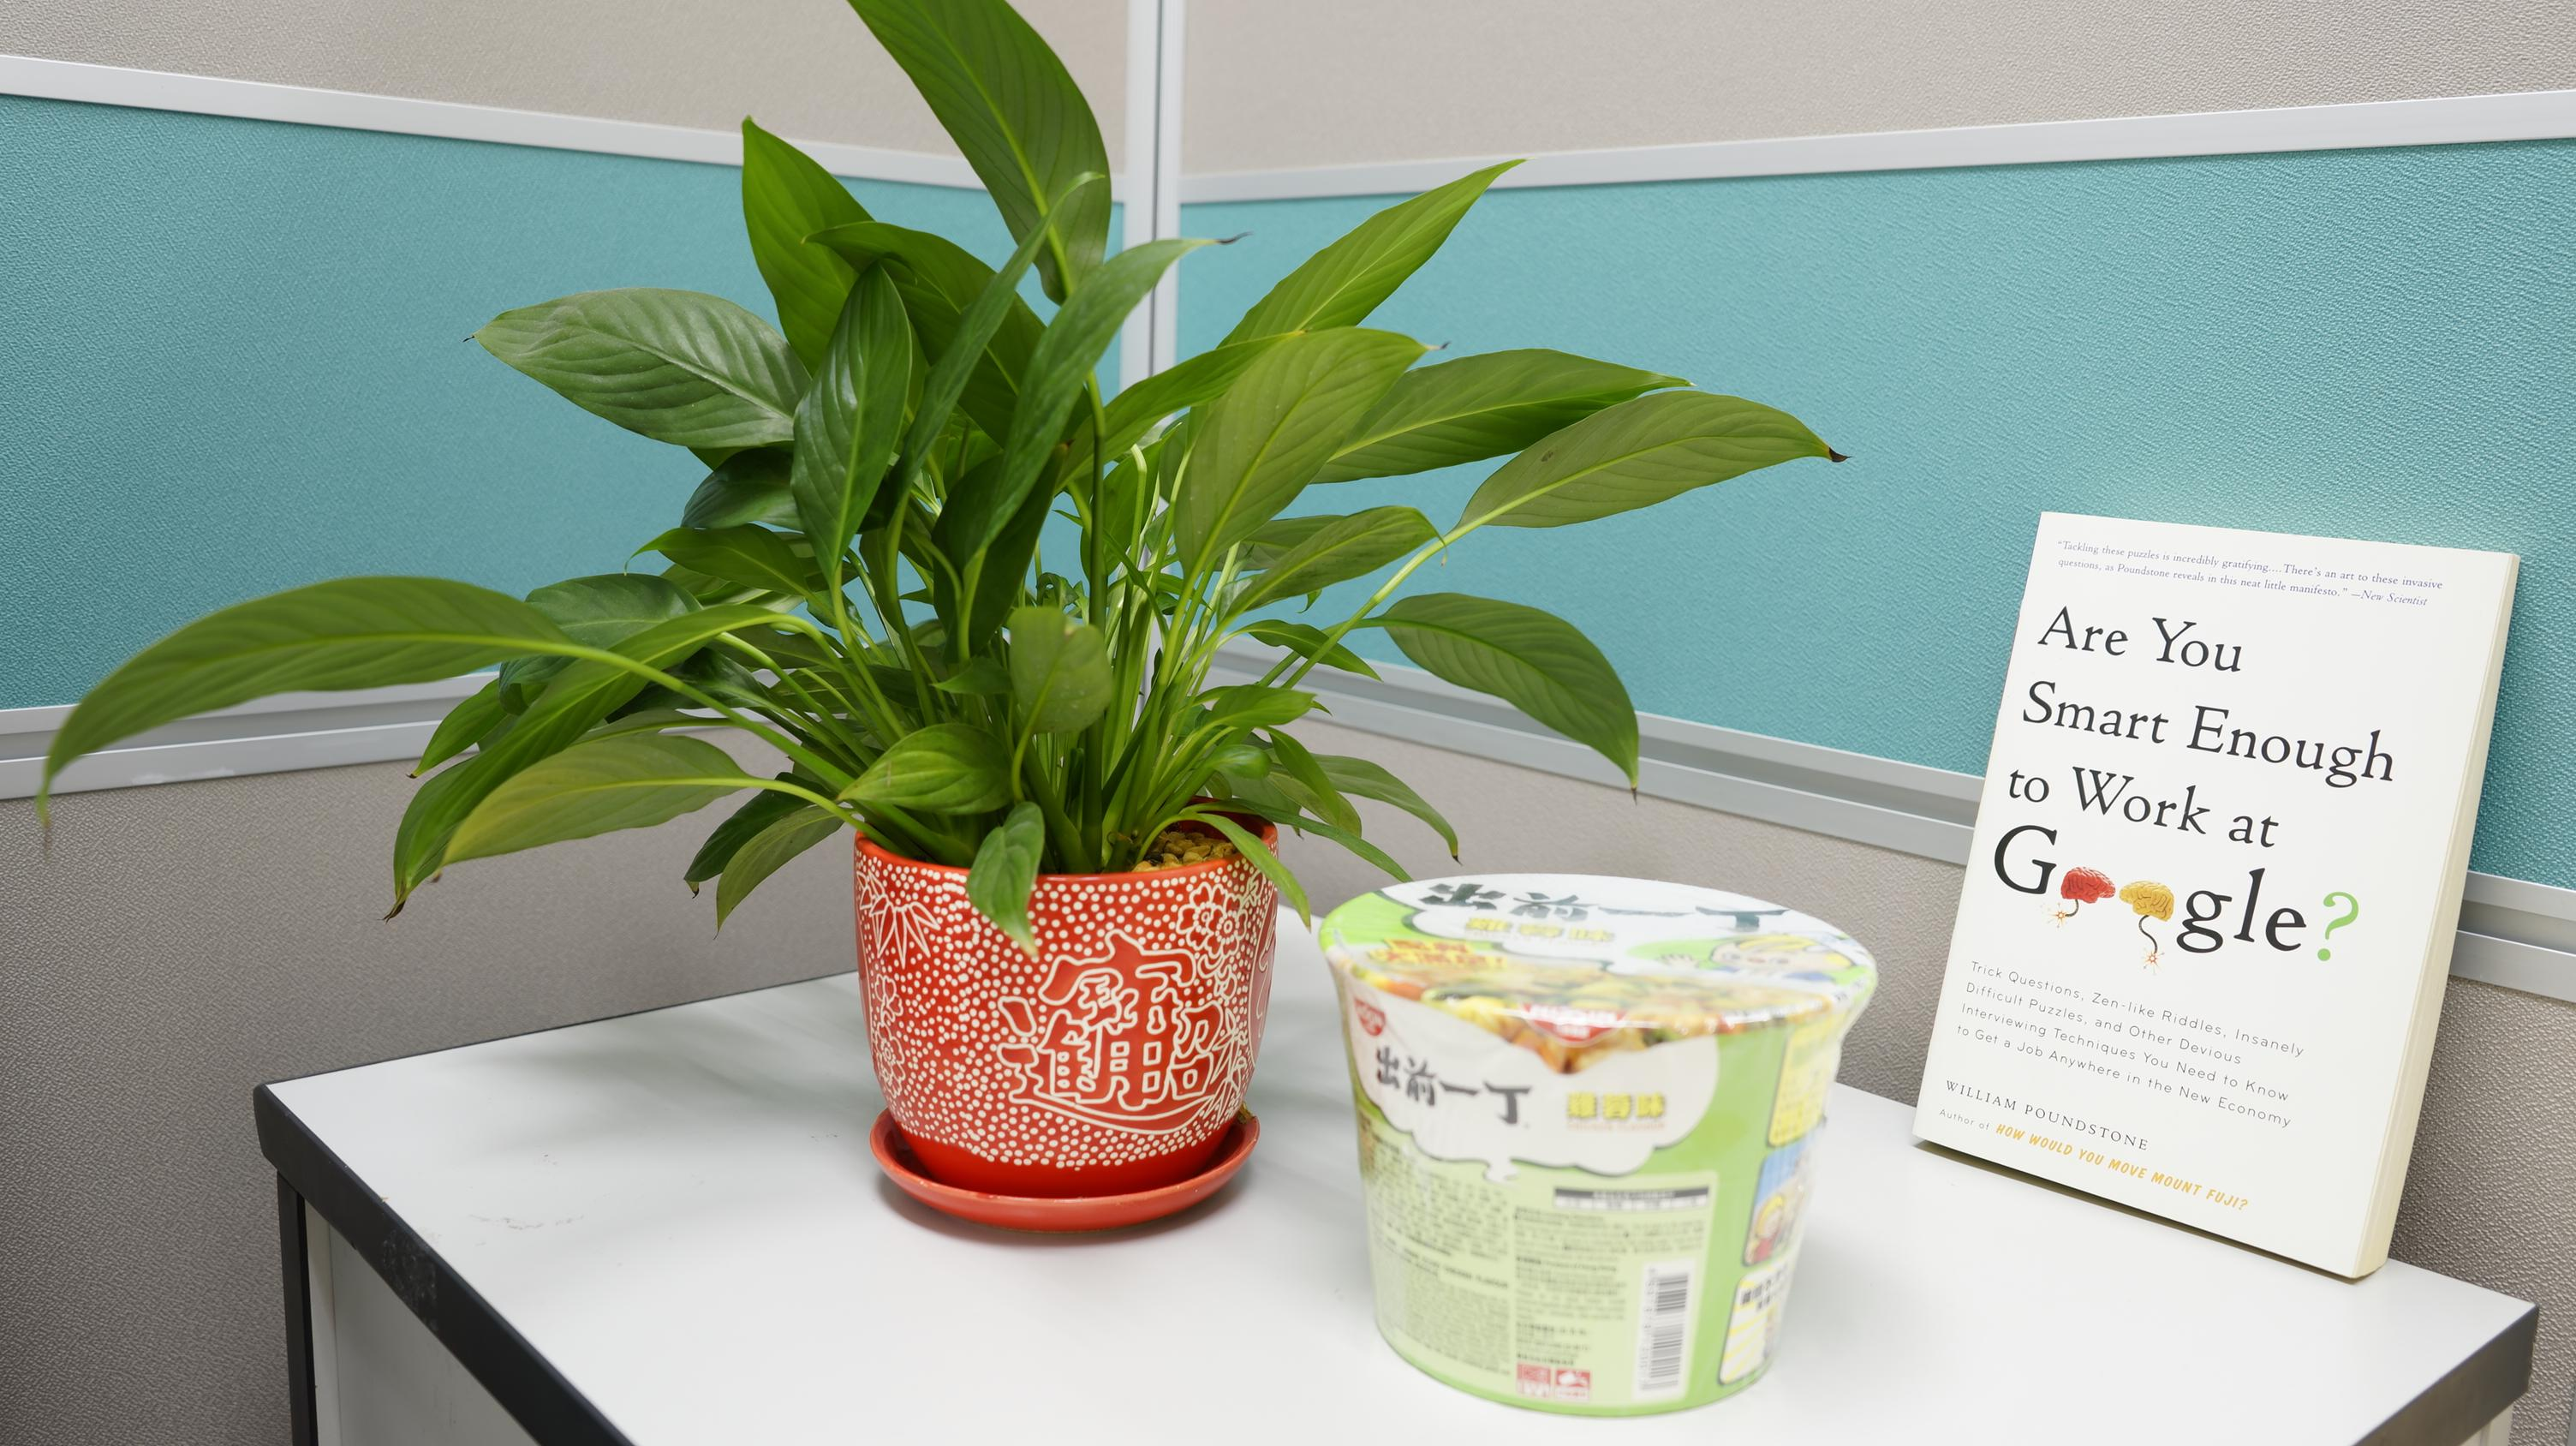
\includegraphics[width=1\textwidth]{images/dataset/Sony_4-5_125_3200_plant_mean.JPG}
    \end{subfigure}
    \hfill
    \begin{subfigure}[t]{0.32\textwidth}
        \centering
        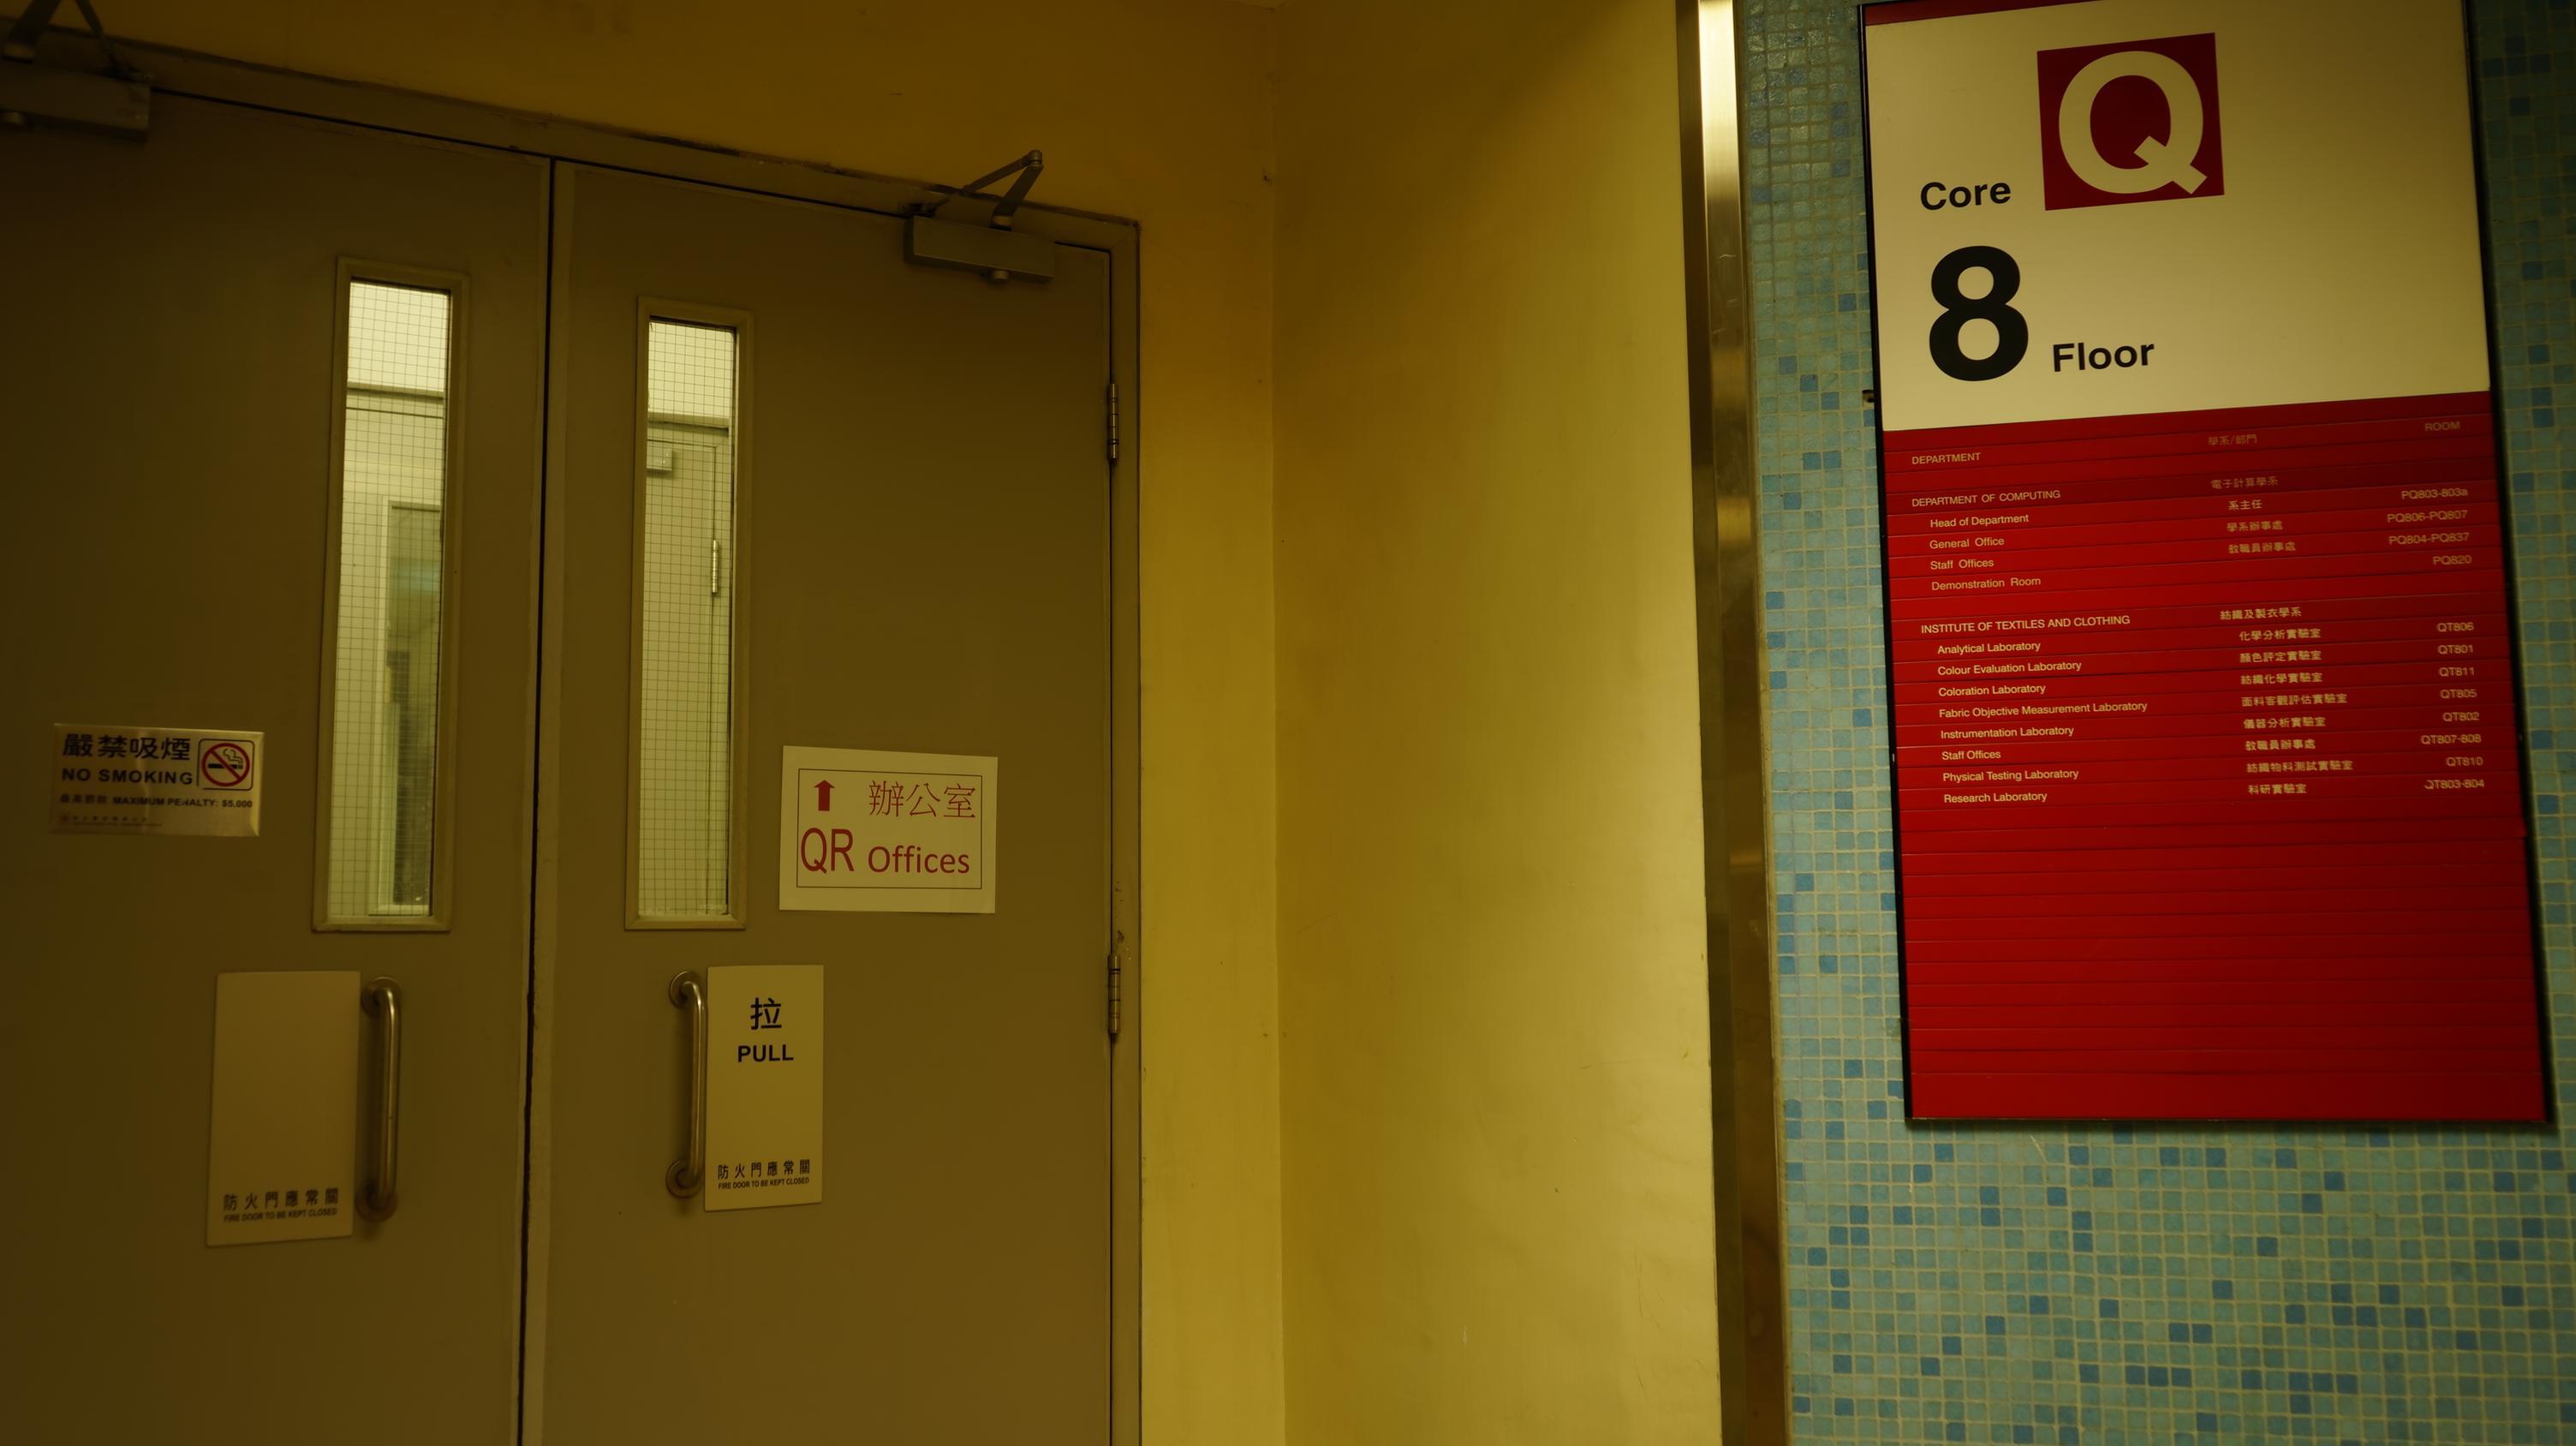
\includegraphics[width=1\textwidth]{images/dataset/Sony_4_200_3200_door_mean.JPG}
    \end{subfigure}
    \hfill
    \begin{subfigure}[t]{0.32\textwidth}
        \centering
        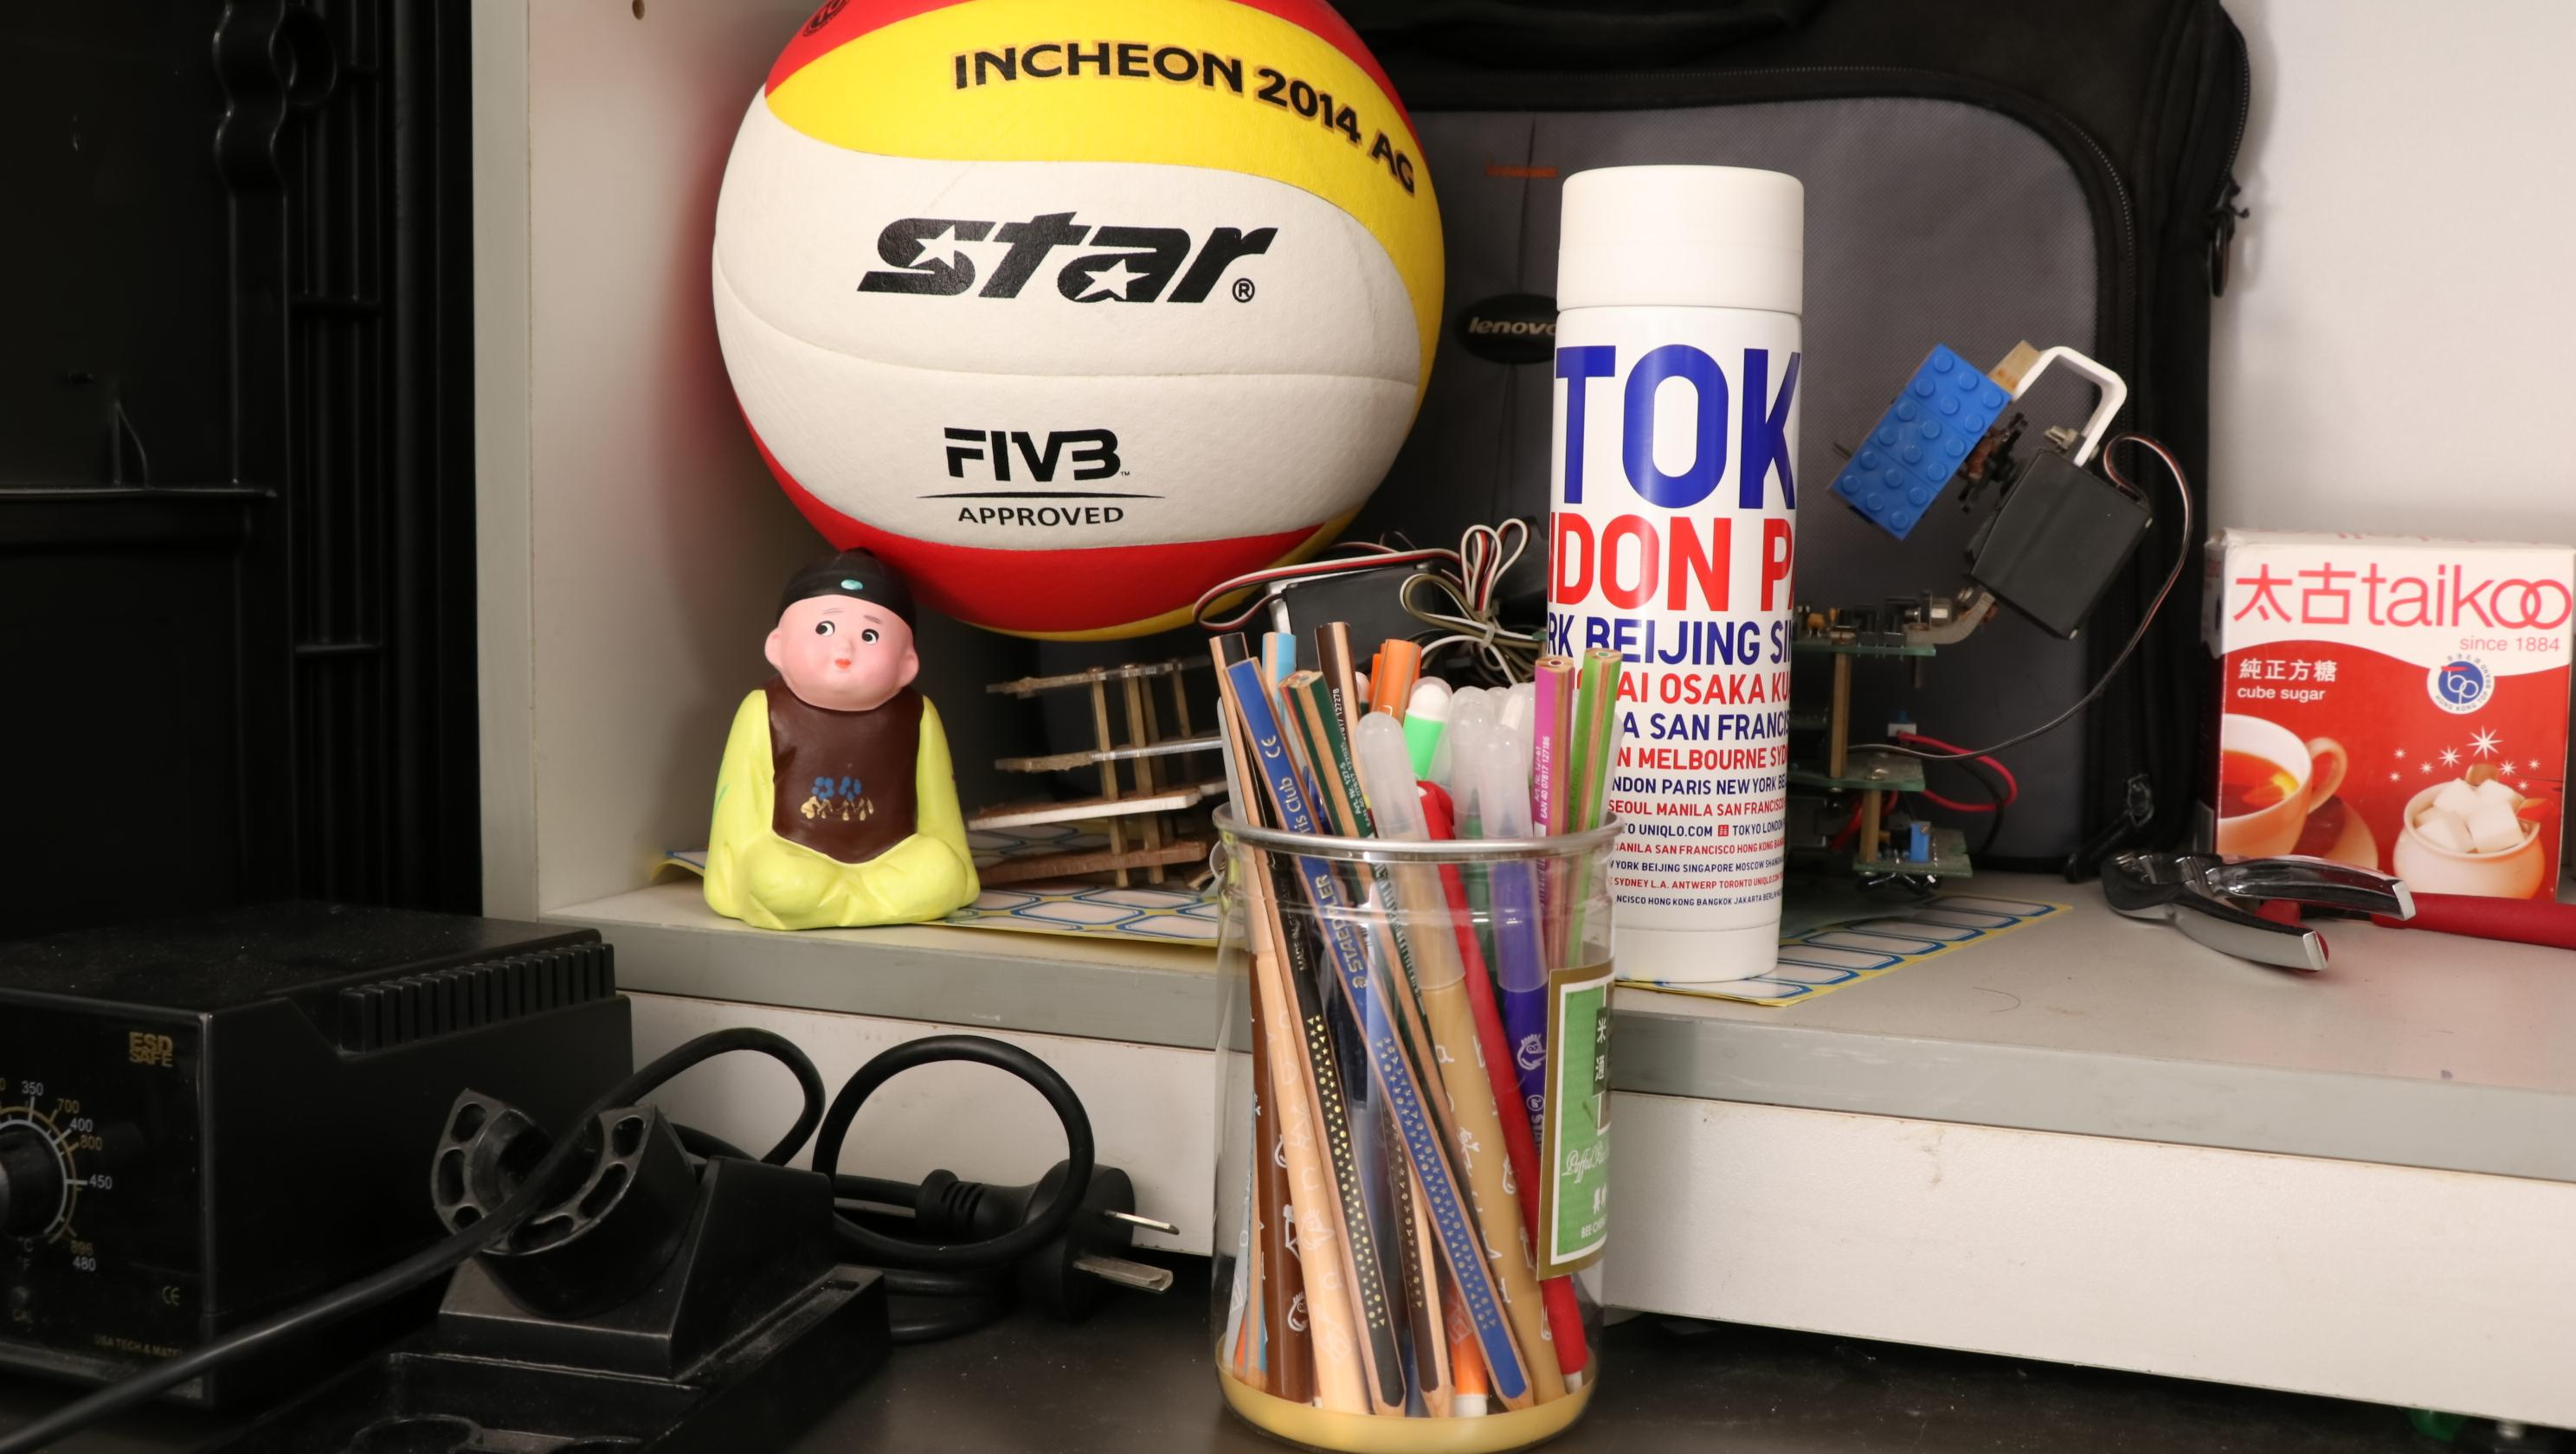
\includegraphics[width=1\textwidth]{images/dataset/Canon80D_8_8_3200_ball_mean.JPG}
    \end{subfigure}
    \hfill
    \begin{subfigure}[t]{0.32\textwidth}
        \centering
        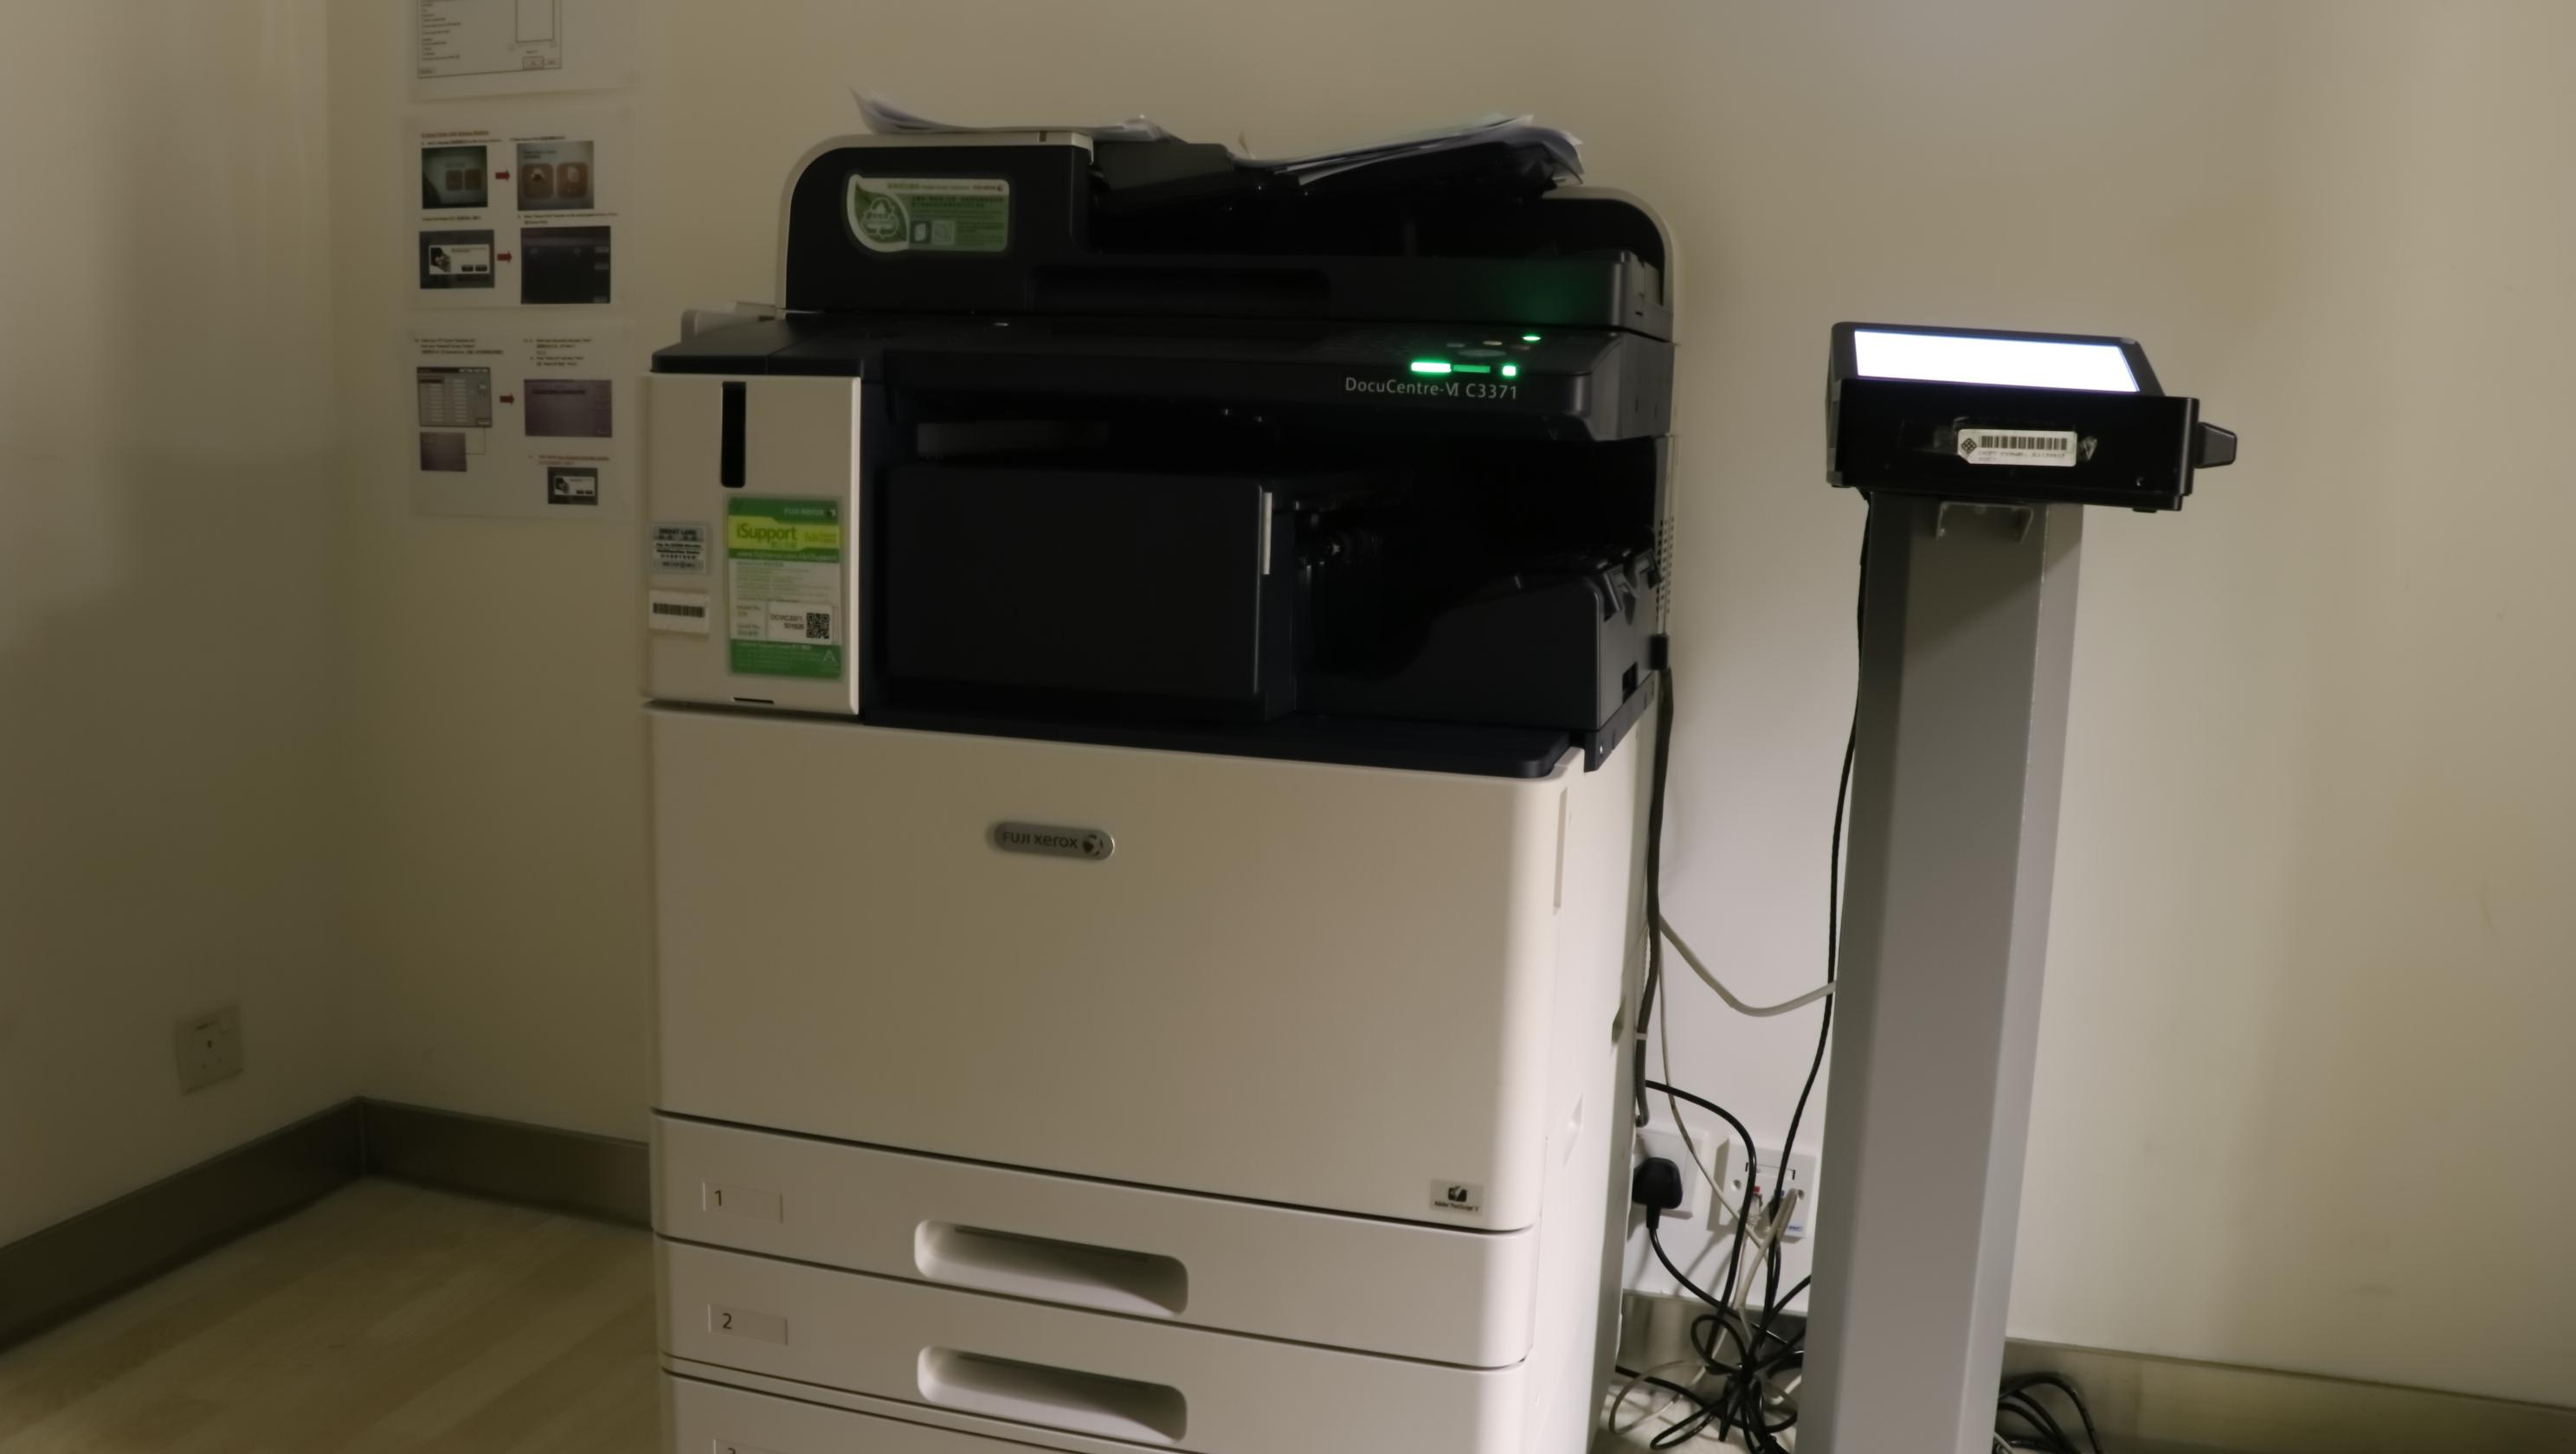
\includegraphics[width=1\textwidth]{images/dataset/Canon80D_8_8_12800_printer_mean.JPG}
    \end{subfigure}
    \hfill
    \begin{subfigure}[t]{0.32\textwidth}
        \centering
        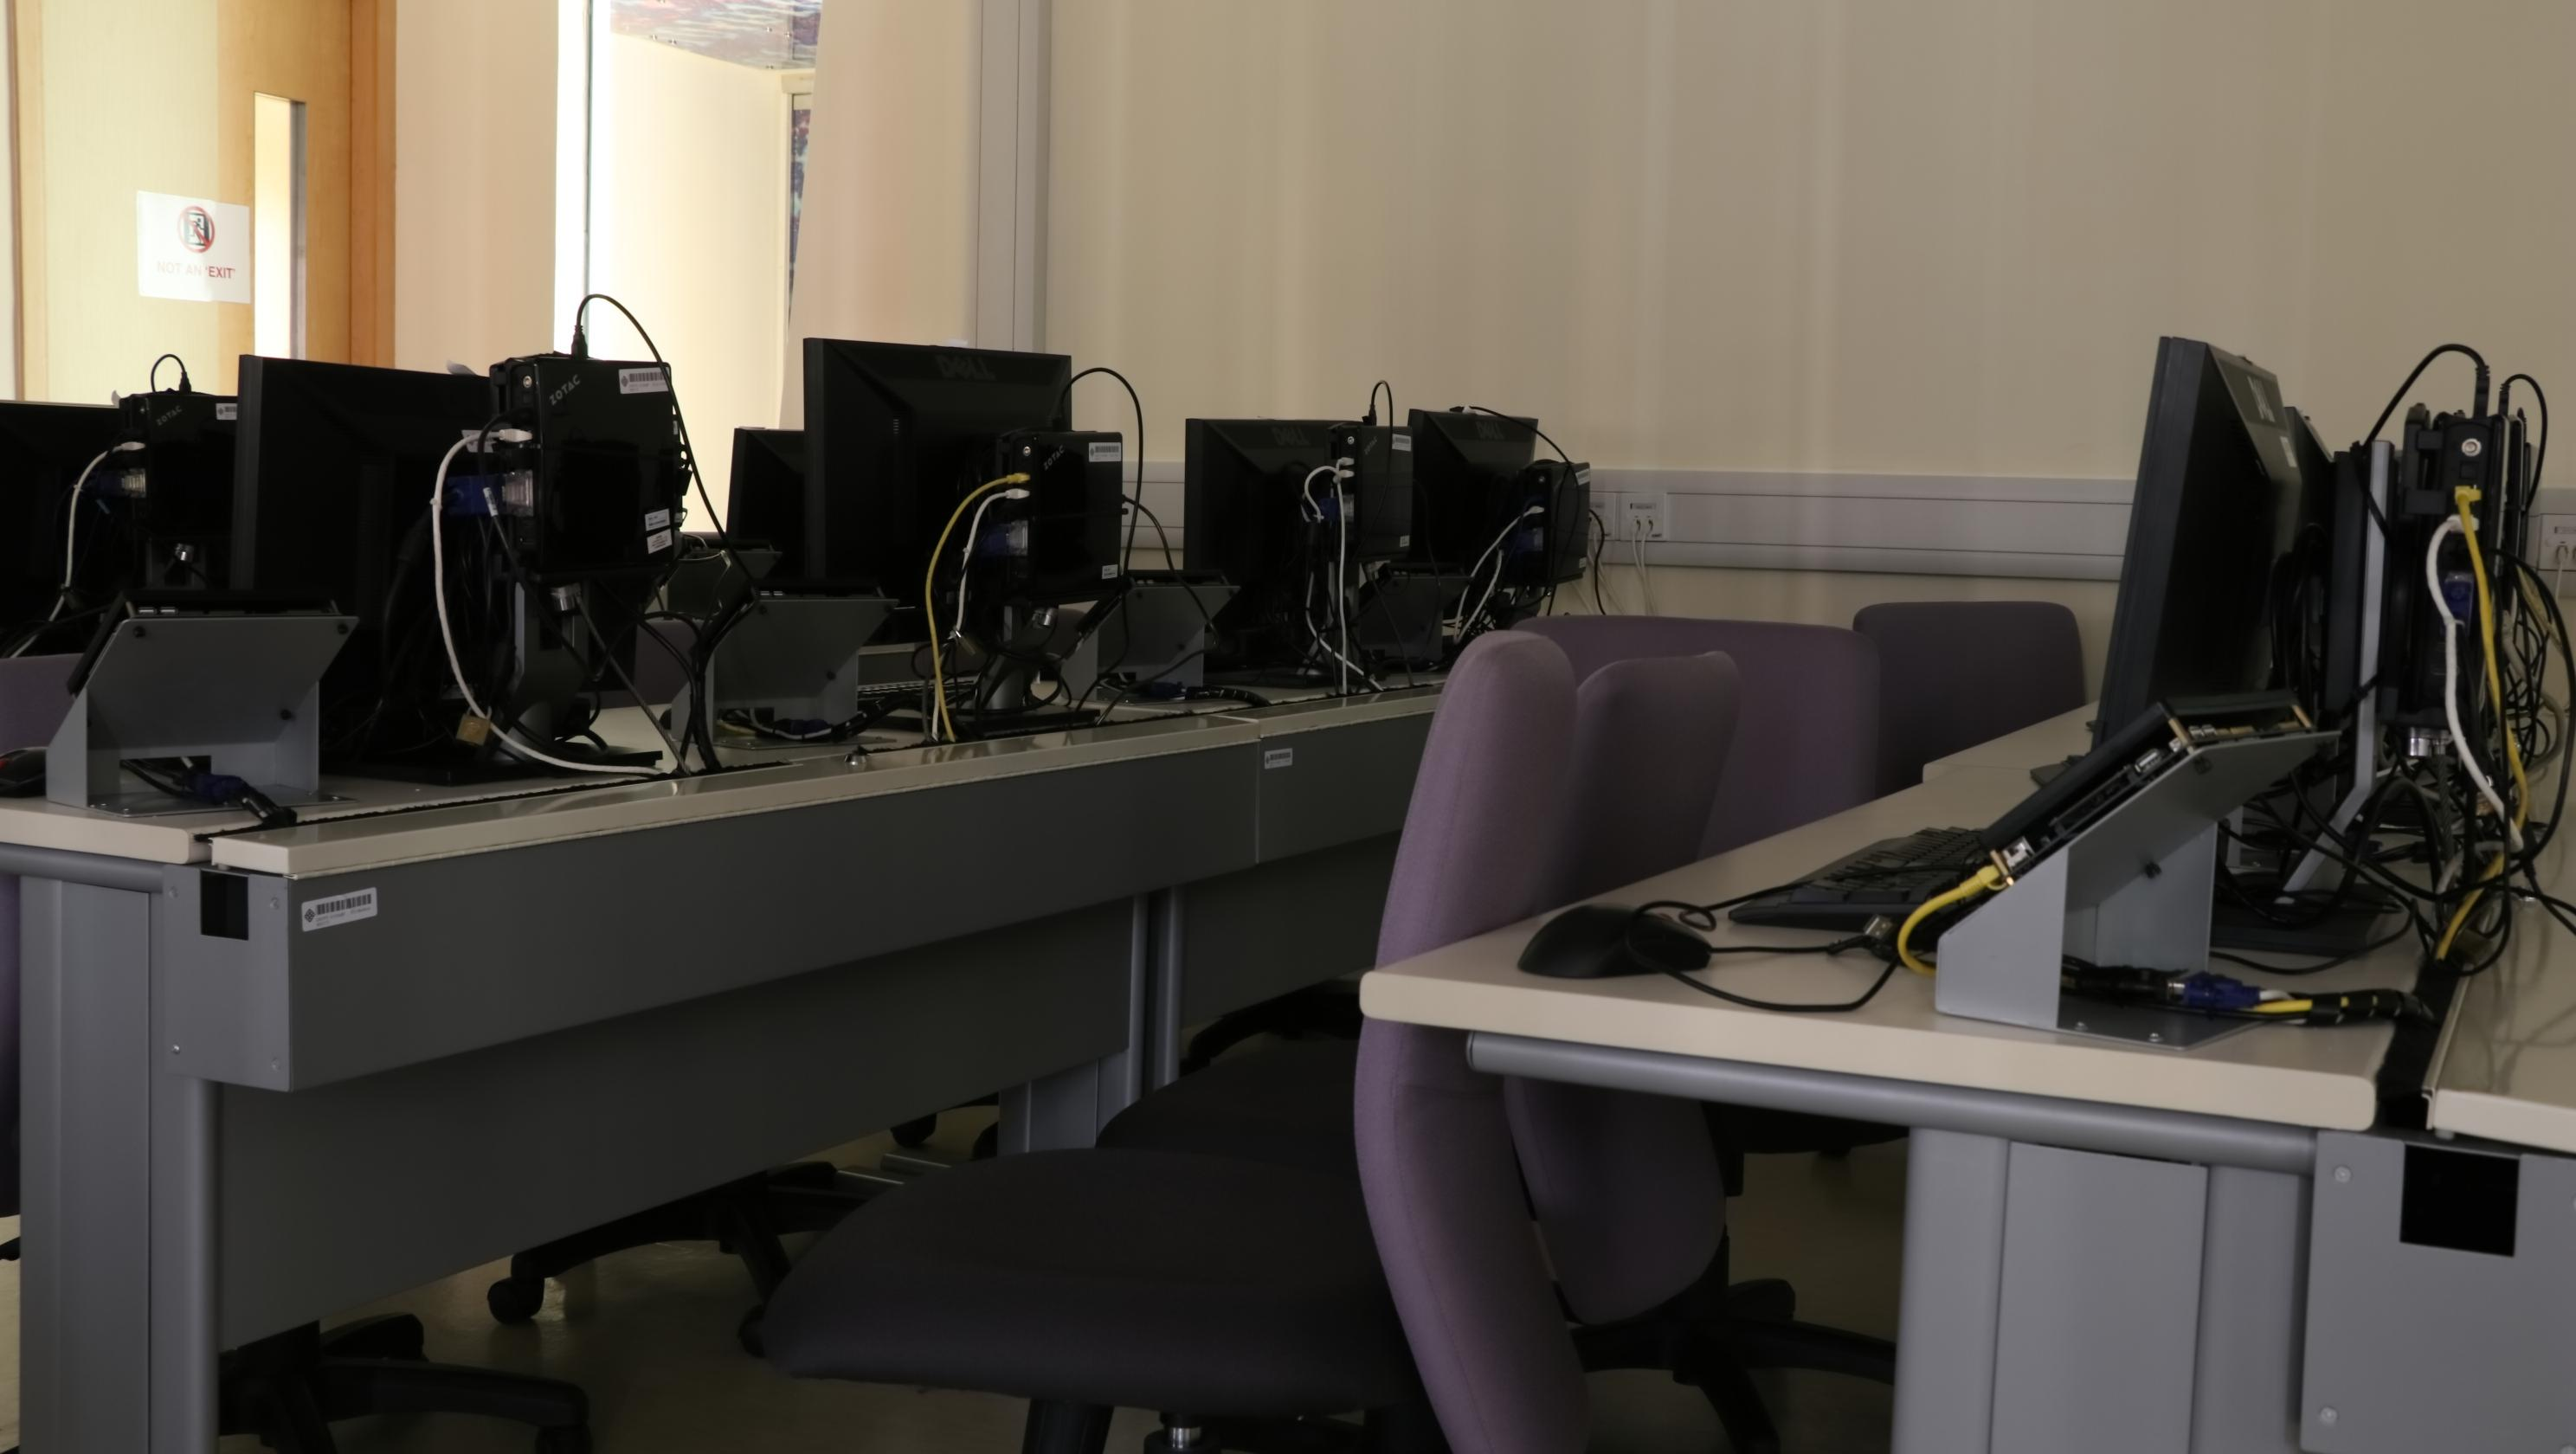
\includegraphics[width=1\textwidth]{images/dataset/Canon80D_8_8_6400_comproom_mean.JPG}
    \end{subfigure}
    \caption{Some examples in our newly constructed dataset.}
    \label{fig6-2}
\end{figure}

\begin{figure}
\centering
    \begin{subfigure}[t]{0.24\textwidth}
        \centering
        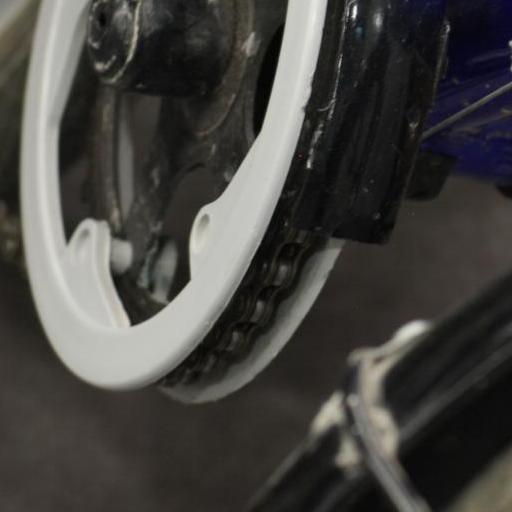
\includegraphics[width=1\textwidth]{images/dataset/Canon5D2_5_160_6400_bicycle_6_mean.JPG}
    \end{subfigure}
\hfill
    \begin{subfigure}[t]{0.24\textwidth}
        \centering
        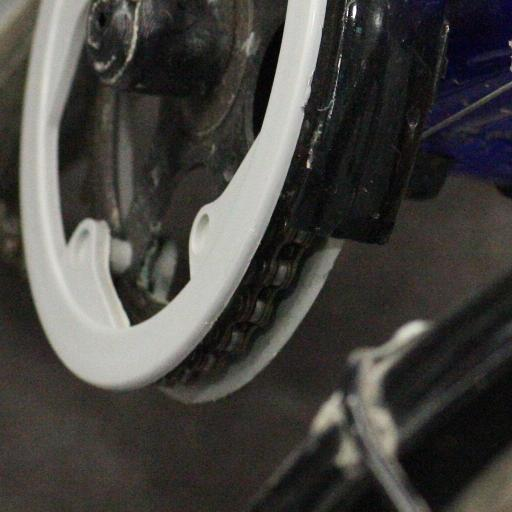
\includegraphics[width=1\textwidth]{images/dataset/Canon5D2_5_160_6400_bicycle_6_real.JPG}
    \end{subfigure}   
\hfill
    \begin{subfigure}[t]{0.24\textwidth}
        \centering
        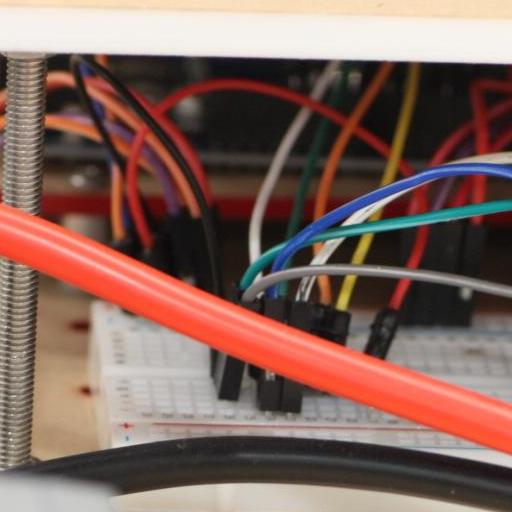
\includegraphics[width=1\textwidth]{images/dataset/Canon5D2_5_160_6400_circuit_11_mean.JPG}
    \end{subfigure}
\hfill
    \begin{subfigure}[t]{0.24\textwidth}
        \centering
        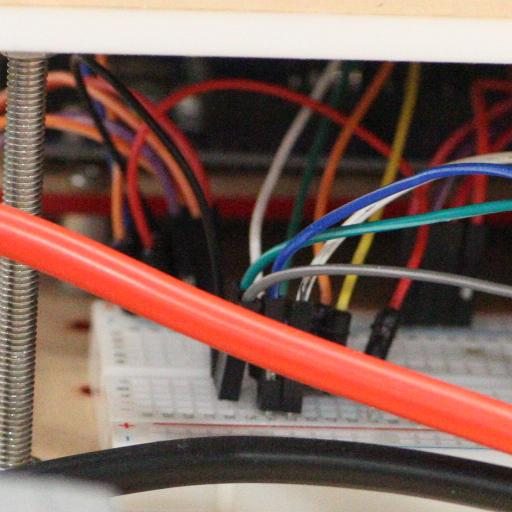
\includegraphics[width=1\textwidth]{images/dataset/Canon5D2_5_160_6400_circuit_11_real.JPG}
    \end{subfigure}

\hfill
    \begin{subfigure}[t]{0.24\textwidth}
        \centering
        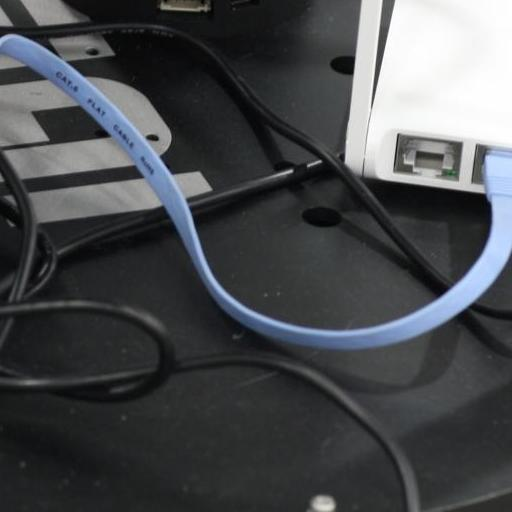
\includegraphics[width=1\textwidth]{images/dataset/Canon5D2_5_160_6400_reciever_1_mean.JPG}
    \end{subfigure} 
\hfill
    \begin{subfigure}[t]{0.24\textwidth}
        \centering
        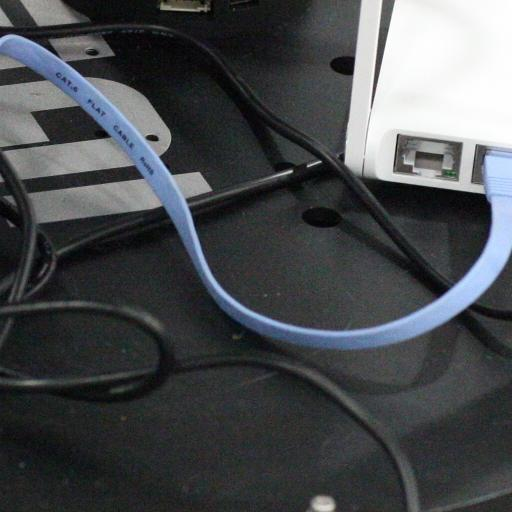
\includegraphics[width=1\textwidth]{images/dataset/Canon5D2_5_160_6400_reciever_1_real.JPG}
    \end{subfigure}
    \hfill
    \begin{subfigure}[t]{0.24\textwidth}
        \centering
        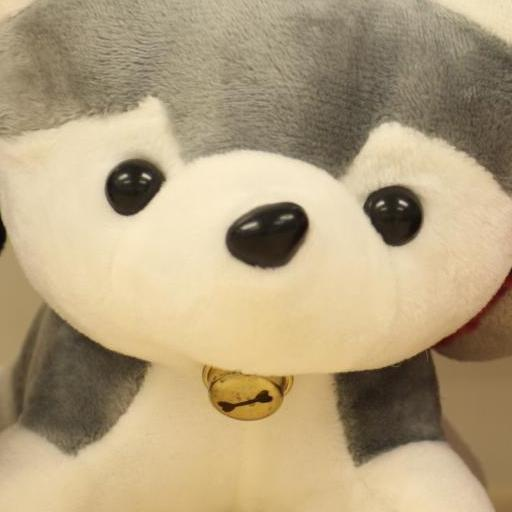
\includegraphics[width=1\textwidth]{images/dataset/Canon5D2_5_200_3200_toy_3_mean.JPG}
    \end{subfigure}
\hfill
    \begin{subfigure}[t]{0.24\textwidth}
        \centering
        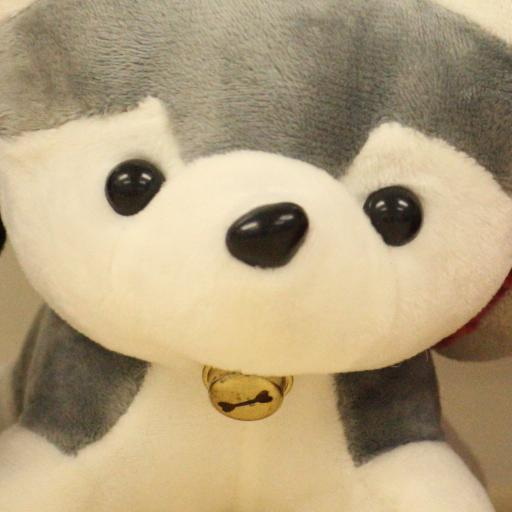
\includegraphics[width=1\textwidth]{images/dataset/Canon5D2_5_200_3200_toy_3_real.JPG}
    \end{subfigure}

\hfill
    \begin{subfigure}[t]{0.24\textwidth}
        \centering
        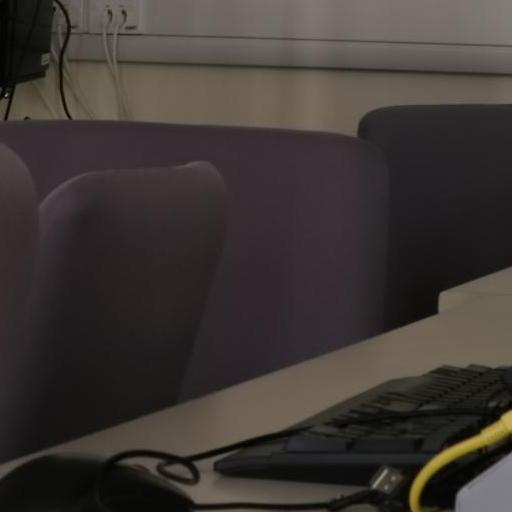
\includegraphics[width=1\textwidth]{images/dataset/Canon80D_8_8_6400_comproom_11_mean.JPG}
    \end{subfigure}
\hfill
    \begin{subfigure}[t]{0.24\textwidth}
        \centering
        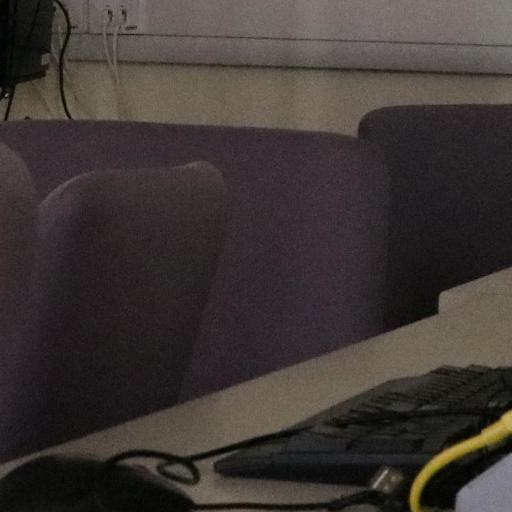
\includegraphics[width=1\textwidth]{images/dataset/Canon80D_8_8_6400_comproom_11_real.JPG}
    \end{subfigure}
\hfill
    \begin{subfigure}[t]{0.24\textwidth}
        \centering
        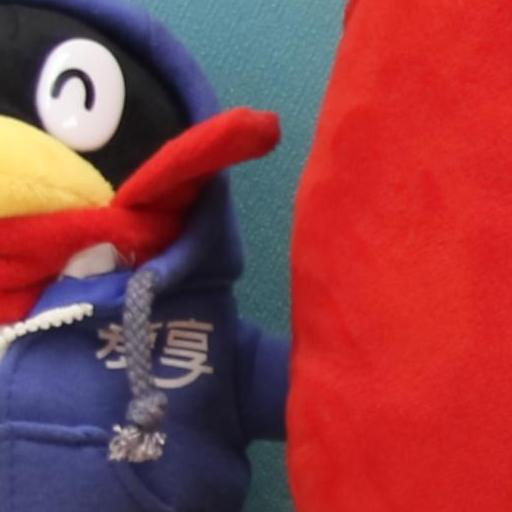
\includegraphics[width=1\textwidth]{images/dataset/Canon600D_4-5_125_1600_toy_16_mean.JPG}
    \end{subfigure}
\hfill
    \begin{subfigure}[t]{0.24\textwidth}
        \centering
        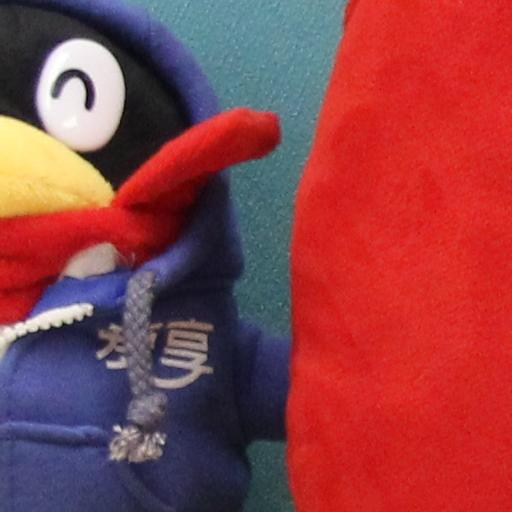
\includegraphics[width=1\textwidth]{images/dataset/Canon600D_4-5_125_1600_toy_16_real.JPG}
    \end{subfigure}

    \hfill
    \begin{subfigure}[t]{0.24\textwidth}
        \centering
        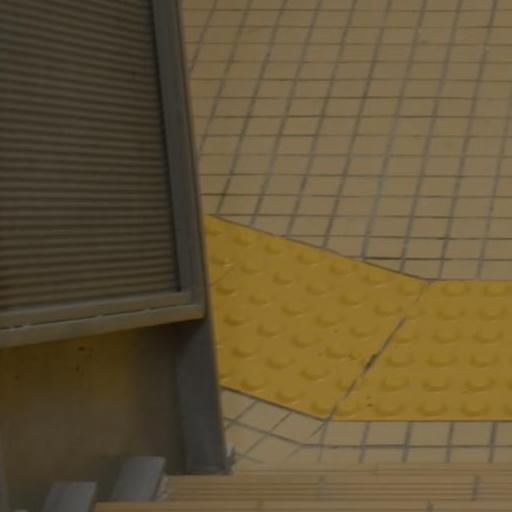
\includegraphics[width=1\textwidth]{images/dataset/NikonD800_5_125_6400_stair_3_mean.JPG}
    \end{subfigure}
     \hfill
    \begin{subfigure}[t]{0.24\textwidth}
        \centering
        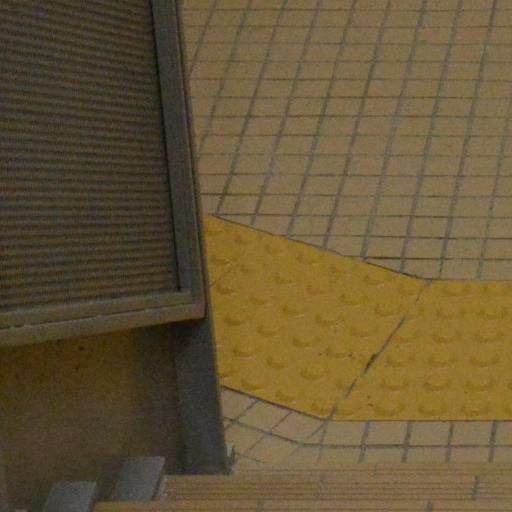
\includegraphics[width=1\textwidth]{images/dataset/NikonD800_5_125_6400_stair_3_real.JPG}
    \end{subfigure}
    \hfill
    \begin{subfigure}[t]{0.24\textwidth}
        \centering
        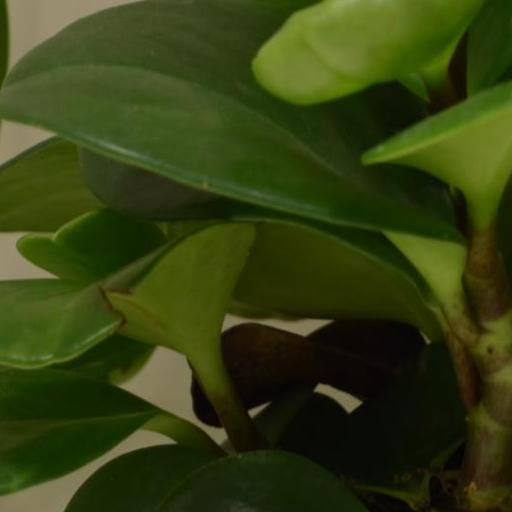
\includegraphics[width=1\textwidth]{images/dataset/NikonD800_6-3_125_5000_plant_1_mean.JPG}
    \end{subfigure}
    \hfill
    \begin{subfigure}[t]{0.24\textwidth}
        \centering
        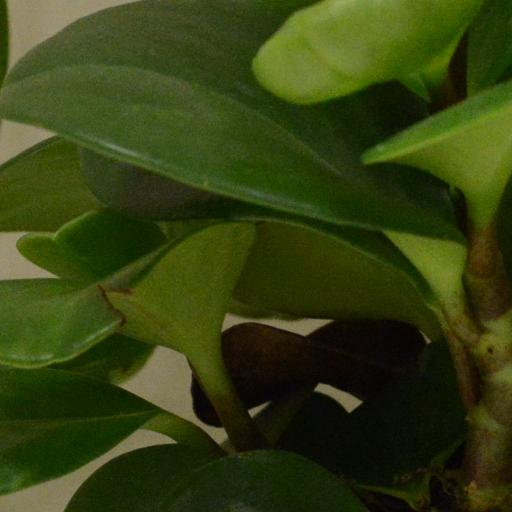
\includegraphics[width=1\textwidth]{images/dataset/NikonD800_6-3_125_5000_plant_1_real.JPG}
    \end{subfigure}


    \hfill
    \begin{subfigure}[t]{0.24\textwidth}
        \centering
        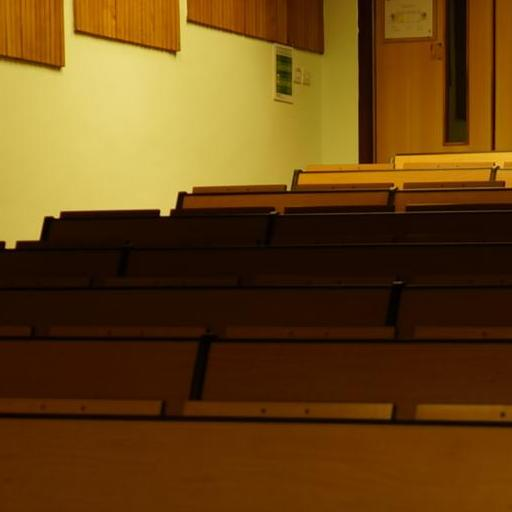
\includegraphics[width=1\textwidth]{images/dataset/Sony_3-5_200_1600_classroom_14_mean.JPG}
    \end{subfigure}
    \hfill
    \begin{subfigure}[t]{0.24\textwidth}
        \centering
        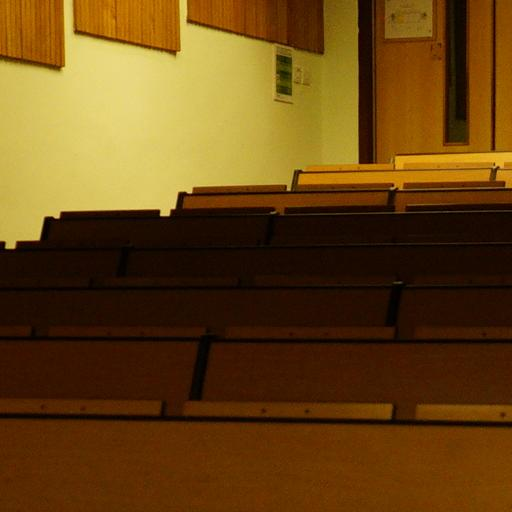
\includegraphics[width=1\textwidth]{images/dataset/Sony_3-5_200_1600_classroom_14_real.JPG}
    \end{subfigure}
    \hfill
    \begin{subfigure}[t]{0.24\textwidth}
        \centering
        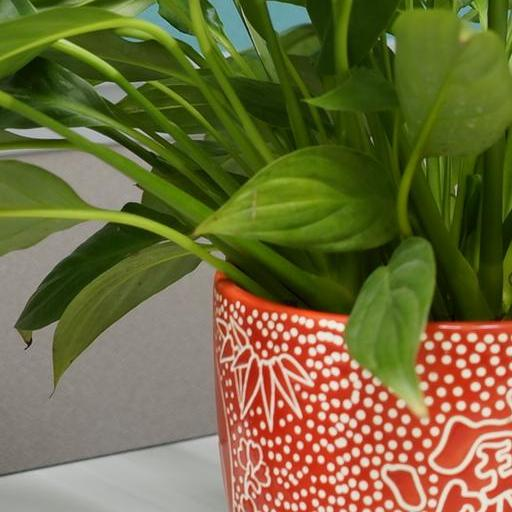
\includegraphics[width=1\textwidth]{images/dataset/Sony_4-5_125_3200_plant_10_mean.JPG}
    \end{subfigure}
    \hfill
    \begin{subfigure}[t]{0.24\textwidth}
        \centering
        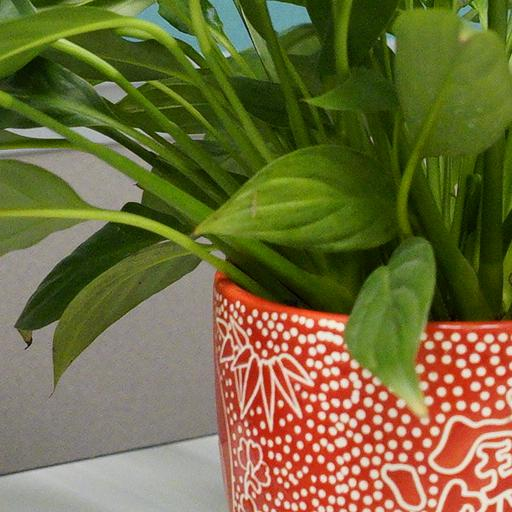
\includegraphics[width=1\textwidth]{images/dataset/Sony_4-5_125_3200_plant_10_real.JPG}
    \end{subfigure}

    \caption{Some cropped parts of the ``ground truth'' images (up) and their corresponding realistic images (down) in our newly constructed dataset.}
    \label{fig6-3}
\end{figure}



\section{Experiments}

\textbf{Benchmark Dataset.} To better illustrate the effectiveness of existing image denising methods, we apply the competing methods on the proposed new dataset. Since many existing methods are very slow in denoising large images (megapixel level), we crop smaller regions of size $512\times512$ pixels from each image in our dataset, yielding overall 100 test images. These images share very small (less than $10\%$) overlap at contents.

\textbf{Comparison methods.} With the proposed dataset, we take a comprehensive evaluation on the state-of-the-art image denoising methods the famous CBM3D \cite{cbm3d}, K-SVD \cite{ksvd}, LSSC \cite{lssc}, Expected Patch Log Likelihood (EPLL) \cite{epll}, multi-layer perception (MLP) \cite{mlp}, Nonlocally Centralized Sparse Representations (NCSR) \cite{ncsr}, Cascades of Shrinkage Fileds (CSF) \cite{csf}, Weighted Nuclear Norm Minimization (WNNM) \cite{wnnm}, Trainable Nonlinear Reactive Diffusion (TNRD) \cite{tnrd}, the residual network based method DnCNN \cite{dncnn}, the ``Noise Clinic'' method \cite{noiseclinic,ncwebsite}, the commercial software Neat Image \cite{neatimage}, and our proposed methods Patch Group Prior based Denoising (PGPD) \cite{pgpd}, external prior guided internal prior learning for image denoising (Guided) \cite{guided}, Multi-channel Weighted Nuclear Norm Minimization (MCWNNM) \cite{mcwnnm}, the Trilateral Weighted Sparse Coding (TWSC) \cite{twsc}. The method of CBM3D is a state-of-the-art color image denoising method, which assumes that the noise is addtive white Gaussian nosie (AWGN). The BM3D, K-SVD, LSSC, EPLL, NCSR, CSF, WNNM, TNRD, DnCNN are state-of-the-art methods for AWGN noise removal on greyscale images, and we apply these methods on each channel of the realsitic color images.  The ``Noise Clnic'' (NC) is a blind image denoising method while Neat Image (NI) is a set of commercial software for image denoising, which has been embedded into Photoshop and Corel Paint Shop. Besides, the method of DnCNN \cite{dncnn} can also deal with realistic noisy images. Our proposed methods includes PGPD, Guided, MCWNNM, and TWSC. The PGPD is proposed for AWGN noise, while the Guided, MCWNNM, and TWSC are proposed for realistic noisy image denoising.

\textbf{Noise level of comparison methods.} For the CBM3D method, the standard deviation of noise on color images should be given as a parameter. For methods of WNNM, MLP, CSF, and TNRD, the noise level in each color channel should be input. For the DnCNN method, it is trained to deal with noise in a range of levels $0\sim55$. We retrain the models of discriminative denoising methods MLP, CSF, and TNRD (using the released codes by the authors) at different noise levels from $\sigma=5$ to $\sigma=50$ with a gap of 5. The denoising is performed by processing each channel with the model trained at the same (or nearest) noise level. The noise levels ($\sigma_{r}, \sigma_{g}, \sigma_{b}$) in R, G, B channels are assumed to be Gaussian and can be estimated via some noise estimation methods \cite{noiselevel,Chen2015ICCV}. In this paper, we employ the method \cite{noiselevel} to estimate the noise level for each color channel.


\textbf{Experimental Results and Discussion.}
The PSNR and SSIM \cite{ssim} results on the 100 cropped images are listed in Table \ref{tab6-1}. We can see that the traditional methods proposed for additive white Gaussian noise are no longer effective enough for the realistic noisy images. The discriminative methods achieve slightly better performance than the traditional methods, while still being inferior than the methods designed for realistic nosiy images.

Some visual comparisons are listed in Figures \ref{fig6-4}-\ref{fig6-13}, from which one can see that our proposed TWSC method removes the noise while still maintains the details. This is because that the TWSC considers different noise levels for each local patch as well as each channel. Hence, the TWSC can adaptively process each local region of the noisy images according to the noise level in that region. This property makes the proposed TWSC method more flexible than the other state-of-the-art image denoising methods. 

Contrast to the proposed methods, the traditional denoising methods (e.g., LSSC, EPLL, NCSR, WNNM, and PGPD) designed for grey scale image would generate artifacts since they process each channel of the RGB image individually \cite{srcolor}. They cannot deal with the images which have different noise statistics in different channels as well as different local region. Hence, these methods would fail to process the realistic noisy images captured from real-world scenes. On the other hand, the discriminative learning based methods (e.g., MLP, CSF, TNRD, and DnCNN) are trained on paired clean and noisy images. These methods largely depends on the training dataset, and would achieve inferior performance upon the noise in the testing images is different from the noise in the training images.

\begin{table}[hbp]
\caption{Average results on PSNR(dB) and SSIM of different denoising algorithms on the 100 cropped images in our new dataset.}
\scriptsize
\label{tab6-1}
\begin{center}
\renewcommand\arraystretch{1.2}
\begin{tabular*}{1\textwidth}{@{\extracolsep{\fill}}ccccccccc}
\hline
Metric
&
\textbf{CBM3D}
&
\textbf{KSVD}
&
\textbf{LSSC}
&
\textbf{EPLL}
&
\textbf{NCSR}
&
\textbf{WNNM}
&
\textbf{MLP}
&
\textbf{CSF}
\\
\hline
PSNR & 37.40 & 36.29 &  & 36.17 & 36.40 & 31.59 & 38.07 & 37.71
\\
\hline
SSIM & 0.9526 & 0.9255 &  & 0.9216 & 0.9290 & 0.8347 & 0.9615 & 0.9571
\\
\hline
Metric
&
\textbf{TNRD}
&
\textbf{DnCNN}
&
\textbf{NC}
&
\textbf{NI}
&
\textbf{PGPD}
&
\textbf{Guided}
&
\textbf{MCWNNM}
&
\textbf{TWSC}
\\
\hline
PSNR & 38.17 & 36.08 &  &  & 36.18 & 38.35 & 38.51 & \textbf{38.60}
\\
\hline
SSIM & 0.9640 & 0.9161 &  &  & 0.9206 & 0.9669 & 0.9671 & \textbf{0.9685}
\\
\hline
\end{tabular*}
\end{center}
\end{table}




\section{Conclusion}

To evaluate the existing denoising algorithms on real photographs and further promote new emerging algorithms for processing realistic noise, we construct a novel dataset which contains comprehensive realistic noisy images of different natural scenes. These images are captured by different cameras under different camera settings. I first select the baseline image by computing the average image. Then I delete the images which are not in consistant illumiance with the baseline image. Finally, I delete the images which are in misalignment with the baseline images. The whole process are reasonable with rational operations. I use the 500 images which are close to the baseline image on illuminance. Since the captured images are too large, we cropped smaller region of size $512\times512$ to evaluate the existing denoising methods and the methods we proposed in the previous sections. The whole constructed dataset includes 40 different scenes with 100 cropped smaller region.

I take comprehensive study on the denoising experimental results by evaluating the existing state-of-the-art denoising methods with our proposed methods. The results demonstrate that the proposed methods are more robust to the existing competing methods on the newly proposed dataset. The experiments also show the effectiveness and efficiency of our proposed TWSC method. We will make the constructed dataset of real photographs publicly available as another benchmark for implementing the exitsing datasets. What's more, our analysis reveals that the existing scientific practice for the image denoising problem is rather limited, and the existing image quality assessment has rather limited relevance for the realistic settings, both of which need huge potential as well as demand for future research.





















